\documentclass[11pt,a4paper]{article}

% ----------------------------------------------------
% PACKAGES ESSENTIELS
% ----------------------------------------------------
\usepackage[utf8]{inputenc}        % Encodage du texte (UTF-8)
\usepackage[T1]{fontenc}           % Encodage des caractères français
\usepackage[english]{babel}         % Langue du document
\usepackage{geometry}              % Gestion des marges
\usepackage{graphicx}              % Insertion d’images
\usepackage{amsmath, amssymb}      % Symboles et équations mathématiques
\usepackage{siunitx}               % Unités du Système International (SI)
\usepackage{caption}               % Amélioration des légendes
\usepackage{subcaption}            % Sous-figures
\usepackage{booktabs}              % Tableaux esthétiques
\usepackage{float}                 % Contrôle de la position des figures
\usepackage{hyperref}              % Liens cliquables dans le PDF
\usepackage{xcolor}                % Gestion des couleurs
\usepackage{fancyhdr}              % En-têtes et pieds de page personnalisés
\usepackage{enumitem}              % Listes personnalisées
\usepackage{physics}               % Notation physique (contraintes, déformations, etc.)
\usepackage{listings}
\usepackage{xcolor} % Requis pour la coloration syntaxique
\usepackage{tabularx}
\usepackage{booktabs}
\usepackage{multicol}
% ----------------------------------------------------
% PARAMÈTRES DE MISE EN PAGE
% ----------------------------------------------------
\geometry{margin=2.5cm}            % Marges du document
\setlength{\parskip}{0.5em}        % Espacement entre les paragraphes
\setlength{\parindent}{0pt}        % Pas d’indentation au début des paragraphes

% SVG
\usepackage{svg}


% Configuration des liens
\hypersetup{
    colorlinks=true,
    linkcolor=blue,
    urlcolor=blue,
    citecolor=gray
}

% ----------------------------------------------------
% COULEURS ENSTA
% ----------------------------------------------------
\definecolor{enstaBleuFonce}{HTML}{003366}   % Bleu marine (sections)
\definecolor{enstaBleuClair}{HTML}{0073CF}   % Bleu moyen (sous-sections)

% ----------------------------------------------------
% STYLE DES SECTIONS
% ----------------------------------------------------
\usepackage{titlesec}

% Section (bleu marine, majuscule, gras)
\titleformat{\section}
  {\normalfont\huge\bfseries\color{enstaBleuFonce}}
  {\thesection}{1em}{}

% Sous-section (bleu clair, gras)
\titleformat{\subsection}
  {\normalfont\large\bfseries\color{enstaBleuClair}}
  {\thesubsection}{1em}{}

% Sous-sous-section en noir mais plus discret
\titleformat{\subsubsection}
  {\normalfont\normalsize\bfseries\color{black!70}}
  {\thesubsubsection}{1em}{}

% Horizontal line
\titleformat{\section}[block]
  {\normalfont\Large\bfseries\color{enstaBleuFonce}}
  {\thesection}{1em}{}
  [\vspace{0.3em}\titlerule\color{enstaBleuFonce}\vspace{0.3em}]


% ----------------------------------------------------
% EN-TÊTES ET PIEDS DE PAGE
% ----------------------------------------------------
\pagestyle{fancy}
\fancyhf{}
\fancyhead[L]{ENSTA Paris}
\fancyhead[R]{Projet II : Indexation vidéo - Découpage en plans}
\fancyfoot[C]{\thepage}



% ----------------------------------------------------
% FANCY QUOTES
% ----------------------------------------------------
% for adjustwidth environment
\usepackage[strict]{changepage}

% for formal definitions
\usepackage{framed}

% environment derived from framed.sty: see leftbar environment definition
\definecolor{formalshade}{rgb}{0.95,0.95,1}

\newenvironment{formal}{%
  \def\FrameCommand{%
    \hspace{1pt}%
    {\color{enstaBleuFonce}\vrule width 2pt}%
    {\color{formalshade}\vrule width 4pt}%
    \colorbox{formalshade}%
  }%
  \MakeFramed{\advance\hsize-\width\FrameRestore}%
  \noindent\hspace{-4.55pt}% disable indenting first paragraph
  \begin{adjustwidth}{}{7pt}%
  \vspace{2pt}\vspace{2pt}%
}
{%
  \vspace{6pt}\end{adjustwidth}\endMakeFramed%
}

% ----------------------------------------------------
% DÉBUT DU DOCUMENT
% ----------------------------------------------------
\begin{document}

    % ====================================================
    % PAGE DE COUVERTURE
    % ====================================================
    \begin{titlepage}
        \centering
        
\includegraphics[width=0.6\textwidth]{logo_ensta.png}\par\vspace{1cm}
        %{\scshape\LARGE ENSTA Paris \par}
        \vspace{2cm}
        {\Large  CSC 4MI06 - Compléments pour l'Analyse d'Images \par}
        \vspace{1.5cm}
        
        
        {\huge\bfseries Projet II \par}
        {\huge\bfseries Indexation vidéo - Découpage en plans \par}
        
        \vspace{1.5cm}
        
        {\Large Letícia Maria Resende  \par}
        {\Large Naomy Isabela Gomes Biaggi \par}
        \vspace{0.5em}
        \vspace{1.5cm}
        {\large \textbf{Professeur: Antoine MANZANERA}  \par}
        \vfill
        \vspace{0.8cm}
        \textbf{Date :} \today \par
        
        \vspace{1cm}
    
    
    \end{titlepage}

    \section*{Introduction}

        Ce projet s'inscrit dans la problématique générale de l'indexation automatique de flux vidéo . L'augmentation massive des contenus multimédias rend indispensable le développement d'outils capables de structurer automatiquement une vidéo afin de faciliter sa navigation, sa recherche et son archivage. L'étape fondamentale de ce processus consiste à découper la vidéo en ses unités sémantiques de base : les plans.
        
        \subsection*{Définition d'un plan et types de transitions}
        
            Un plan est défini mathématiquement et physiquement comme une séquence d'images enregistrée par une seule caméra au cours d'une prise de vue continue. Au sein d'un même plan, la caméra effectue un mouvement cohérent qui peut se traduire par plusieurs types de configurations cinématographiques  :
            
            \begin{itemize}
                \item \textbf{Plan fixe:} Absence de mouvement global de la caméra .
                \item \textbf{Panoramas (Pan/Tilt) :} Rotation de la caméra autour de son axe horizontal ou vertical.
                \item \textbf{Travelling:} Déplacement de la caméra dans l'espace (horizontal, vertical, avant ou arrière).
                \item \textbf{Zoom:} Modification de la distance focale (avant ou arrière) .
            \end{itemize}
            
            Le passage d'un plan à um autre constitue une transition. On distingue deux grandes familles de changements de plan :
            \begin{enumerate}
            \item \textbf{Les transitions abruptes (Cuts) :} Le passage du plan $P_n$ au plan $P_{n+1}$ se fait de manière instantanée, en un seul changement de frame.
            \item \textbf{Les transitions graduelles :} Le passage se fait de manière progressive sur plusieurs frames via des effets numériques tels que le fondu au noir (\textit{fade-out}), l'ouverture en fondu (\textit{fade-in}) ou le fondu enchaîné (\textit{dissolve}).
            \end{enumerate}
            
        \subsection*{Objectifs et approche méthodologique}
        
            L'objectif principal de ce travail est de concevoir, implémenter et évaluer des algorithmes robustes dédiés à la détection automatique de ces changements de plans. Pour ce faire, nous explorerons trois approches complémentaires basées sur le traitement d'images et la vision par ordinateur :
            
            \begin{itemize}
            
                \item \textbf{L'analyse colorimétrique :} Utilisation des histogrammes 2D de chrominance $(u, v)$ dans l'espace de couleur $YUV$ pour mesurer la rupture de continuité spectrale globale entre frames successives .
                \item \textbf{L'analyse dynamique par flot optique:} Exploitation de l'algorithme de Farneback pour calculer un champ de vitesses dense et analyser la distribution géométrique du mouvement via des histogrammes de vitesses $(V_x, V_y)$ .
                \item \textbf{La compensation de mouvement et erreur résiduelle :} Modélisation prédictive de l'image suivante à l'aide du flot optique, suivie d'une mesure de l'entropie de l'image d'erreur résiduelle pour isoler les ruptures temporelles complexes .
            
            \end{itemize}
            
    \section*{Question I}
    
    
    L’objectif de cette première partie du projet est d’étudier l’évolution temporelle des histogrammes chromatiques d’une séquence vidéo afin d’extraire des informations permettant la détection des changements de plan.
    
    Pour chaque image des vidéos étudiées, un histogramme 2D des composantes chromatiques $(u,v)$ dans l’espace colorimétrique YUV est calculé. Les variations de ces histogrammes au cours du temps sont ensuite analysées à l’aide de différentes mesures de distance.
    
    Dans le cas des vidéos monochromes, les composantes chromatiques deviennent peu informatives. Une approche basée sur l’histogramme de luminance est alors utilisée.
    
    % ==================================================
    % YUV COLOR SPACE
    % ==================================================
    
    \subsection*{Espace colorimétrique YUV}
    
    L’espace YUV sépare l’information de luminance et l’information chromatique :
    
    \begin{itemize}
        \item $Y$ : luminance
        \item $U$ et $V$ : composantes chromatiques
    \end{itemize}
    
    Cette représentation est particulièrement adaptée à l’analyse de contenu vidéo car elle permet d’étudier les variations de couleur indépendamment des variations d’intensité lumineuse.
    
    Dans cette étude, seuls les canaux $(U,V)$ sont utilisés pour les vidéos couleur.
    
    % ==================================================
    % HISTOGRAM COMPUTATION
    % ==================================================
    
    \subsection*{Calcul des histogrammes}
    
    Pour chaque image couleur :
    
    \begin{enumerate}
        \item conversion RGB $\rightarrow$ YUV
        \item extraction des composantes $(U,V)$
        \item calcul d’un histogramme 2D normalisé
    \end{enumerate}
    
    Les histogrammes sont normalisés afin d’obtenir une estimation de probabilité jointe des composantes chromatiques.
    
    Pour les vidéos monochromes, un histogramme 1D de luminance est calculé à partir de l’image en niveaux de gris.
    
    % ==================================================
    % COLOR VIDEOS
    % ==================================================
    
    \subsection*{Exemples de vidéos couleur}
    
    Les figures suivantes montrent plusieurs images représentatives ainsi que leurs histogrammes UV associés.
    
    On observe que les histogrammes sont fortement concentrés autour de certaines zones de l’espace chromatique, reflétant la dominante colorimétrique des scènes.
    
    % ==================================================
    % COSMOS
    % ==================================================
    
    \subsubsection*{Cosmos Laundromat}
    
    \begin{figure}[H]
        \centering
        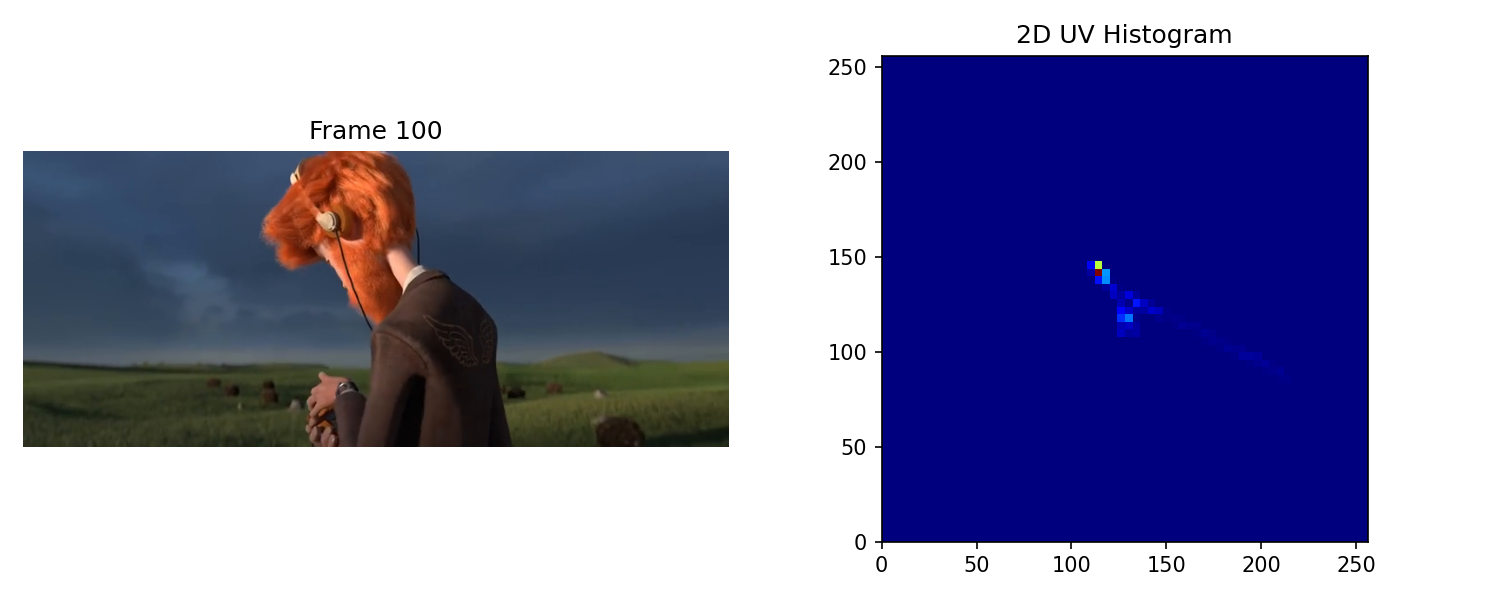
\includegraphics[width=0.9\textwidth]{Images/Extrait1-Cosmos_Laundromat1(340p)_frame_100.png}
        \caption{Exemple d’image et histogramme UV — Cosmos Laundromat (frame 100)}
    \end{figure}
    
    \begin{figure}[H]
        \centering
        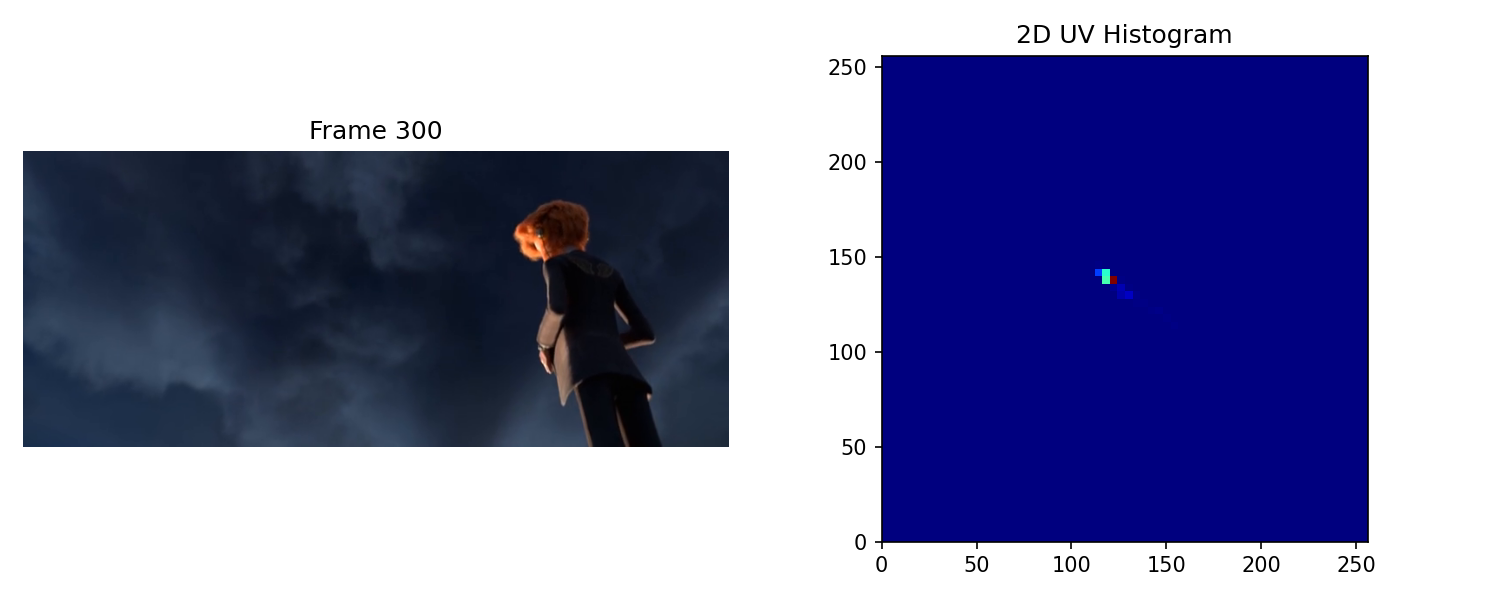
\includegraphics[width=0.9\textwidth]{Images/Extrait1-Cosmos_Laundromat1(340p)_frame_300.png}
        \caption{Exemple d’image et histogramme UV — Cosmos Laundromat (frame 300)}
    \end{figure}
    
    Les histogrammes restent relativement concentrés malgré les variations de contenu de la scène. Les changements de position et d’intensité traduisent les variations chromatiques globales de la séquence.
    
    % ==================================================
    % VERTIGO
    % ==================================================
    
    \subsubsection*{Vertigo Dream Scene}
    
    \begin{figure}[H]
        \centering
        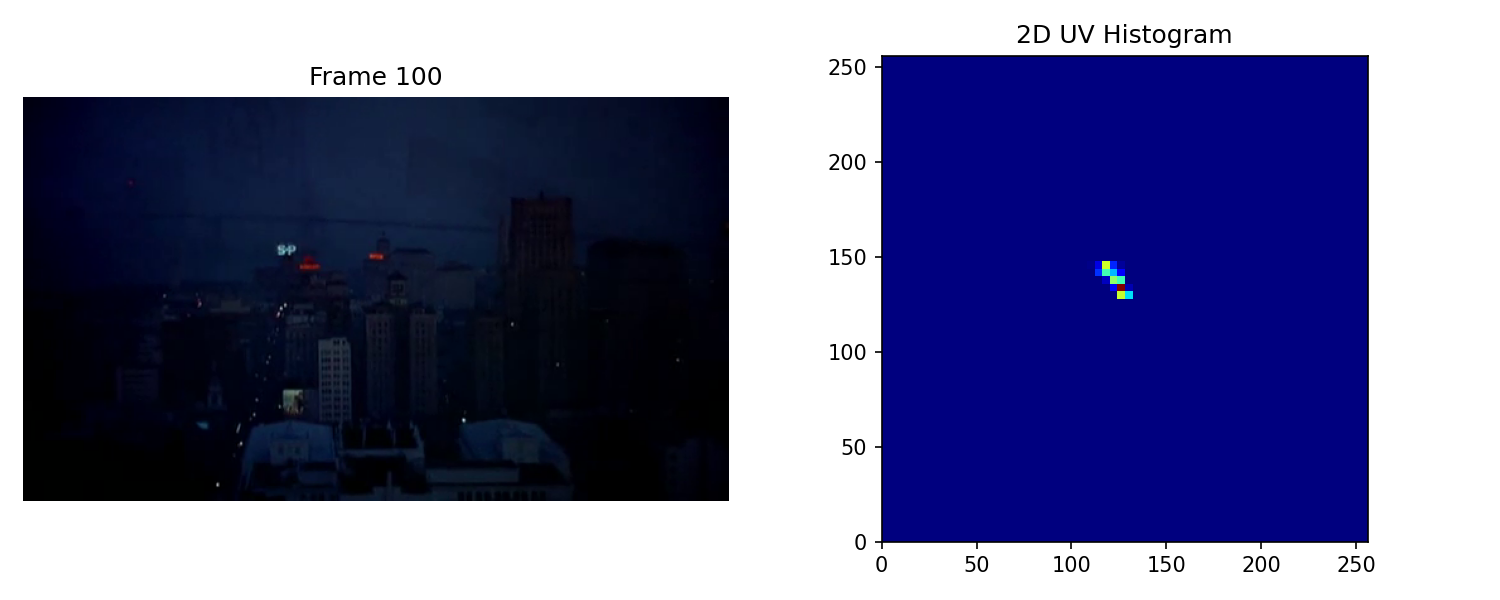
\includegraphics[width=0.9\textwidth]{Images/Extrait3-Vertigo-Dream_Scene(320p)_frame_100.png}
        \caption{Exemple d’image et histogramme UV — Vertigo (frame 100)}
    \end{figure}
    
    \begin{figure}[H]
        \centering
        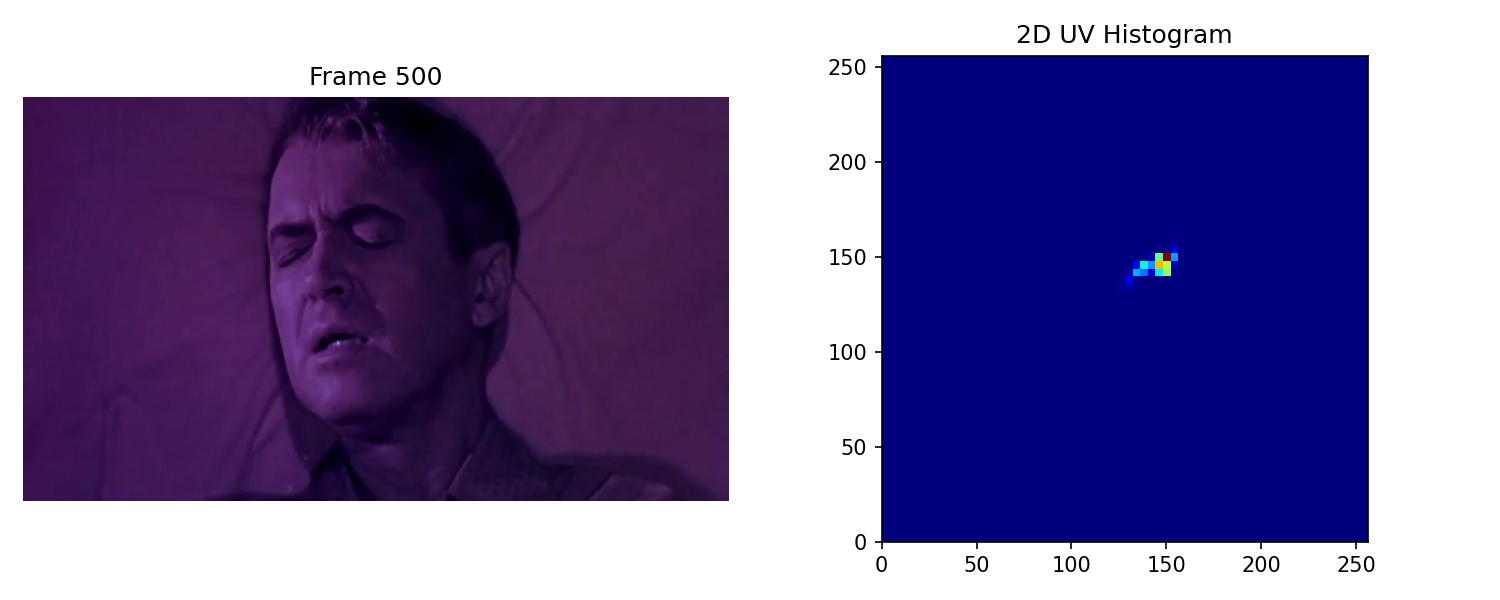
\includegraphics[width=0.9\textwidth]{Images/Extrait3-Vertigo-Dream_Scene(320p)_frame_500.png}
        \caption{Exemple d’image et histogramme UV — Vertigo (frame 500)}
    \end{figure}
    
    Cette séquence présente une forte dominante chromatique violette. Les histogrammes UV sont donc très compacts et fortement localisés dans une région particulière de l’espace chromatique.
    
    % ==================================================
    % MATRIX
    % ==================================================
    
    \subsubsection*{Matrix Helicopter Scene}
    
    \begin{figure}[H]
        \centering
        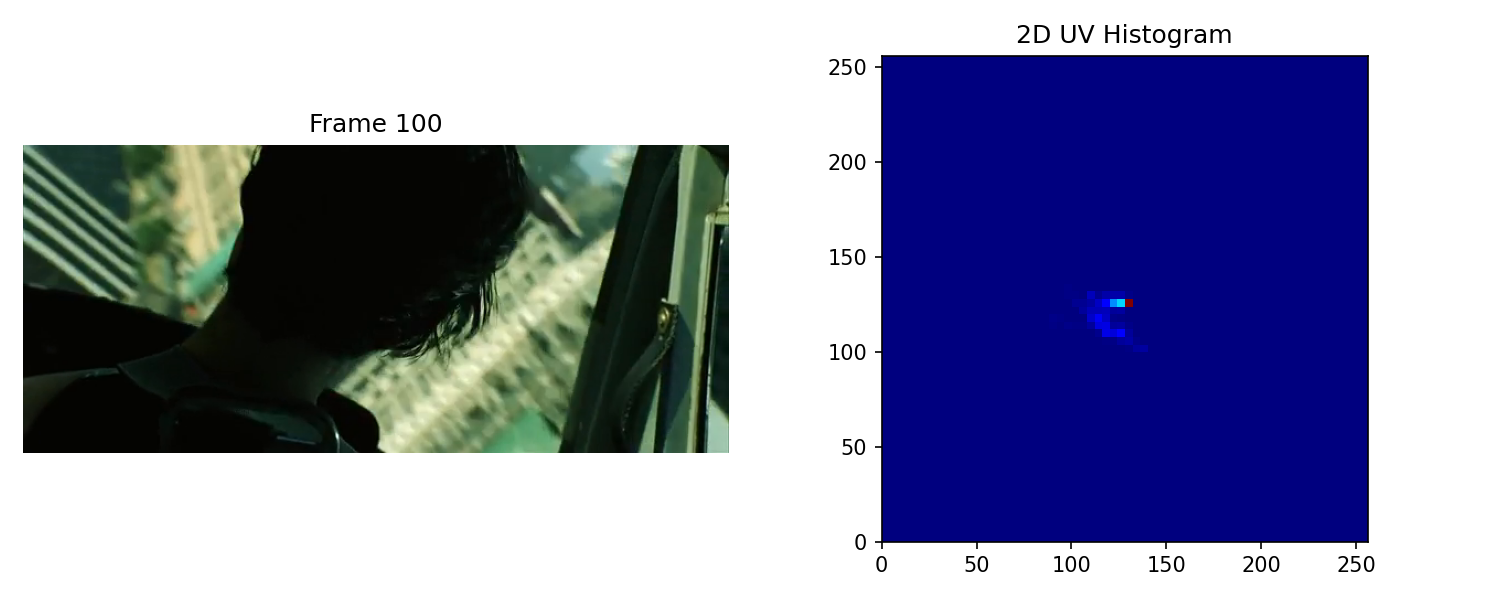
\includegraphics[width=0.9\textwidth]{Images/Extrait5-Matrix-Helicopter_Scene(280p)_frame_100.png}
        \caption{Exemple d’image et histogramme UV — Matrix (frame 100)}
    \end{figure}
    
    \begin{figure}[H]
        \centering
        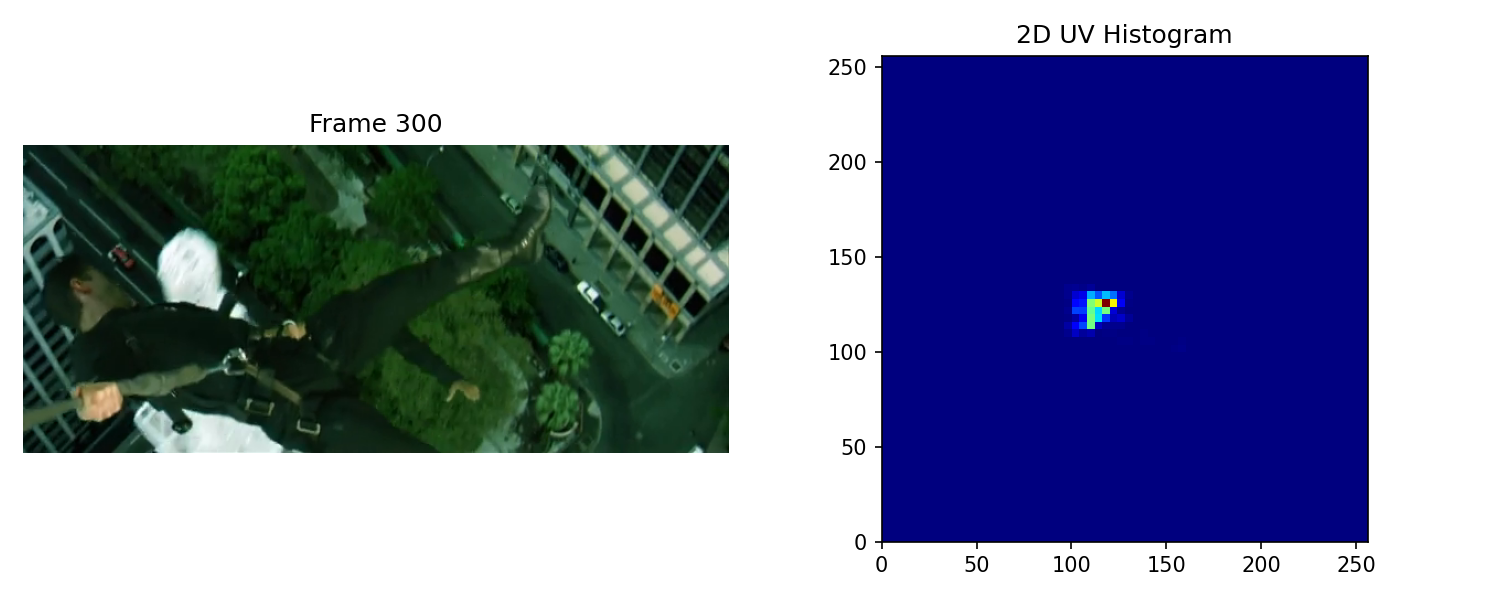
\includegraphics[width=0.9\textwidth]{Images/Extrait5-Matrix-Helicopter_Scene(280p)_frame_300.png}
        \caption{Exemple d’image et histogramme UV — Matrix (frame 300)}
    \end{figure}
    
    La séquence Matrix possède une dominante verdâtre caractéristique. Les histogrammes UV sont davantage étalés que dans le cas de Vertigo, ce qui traduit une plus grande diversité chromatique.
    
    % ==================================================
    % MONOCHROME VIDEOS
    % ==================================================
    
    \subsection*{Cas des vidéos monochromes}
    
    Dans les vidéos monochromes, les composantes chromatiques $(U,V)$ contiennent très peu d’information utile. L’histogramme UV devient alors peu discriminant.
    
    Pour ces séquences, un histogramme de luminance est utilisé à la place.
    
    % ==================================================
    % MAN WITH A MOVIE CAMERA
    % ==================================================
    
    \subsubsection*{Man With A Movie Camera}
    
    \begin{figure}[H]
        \centering
        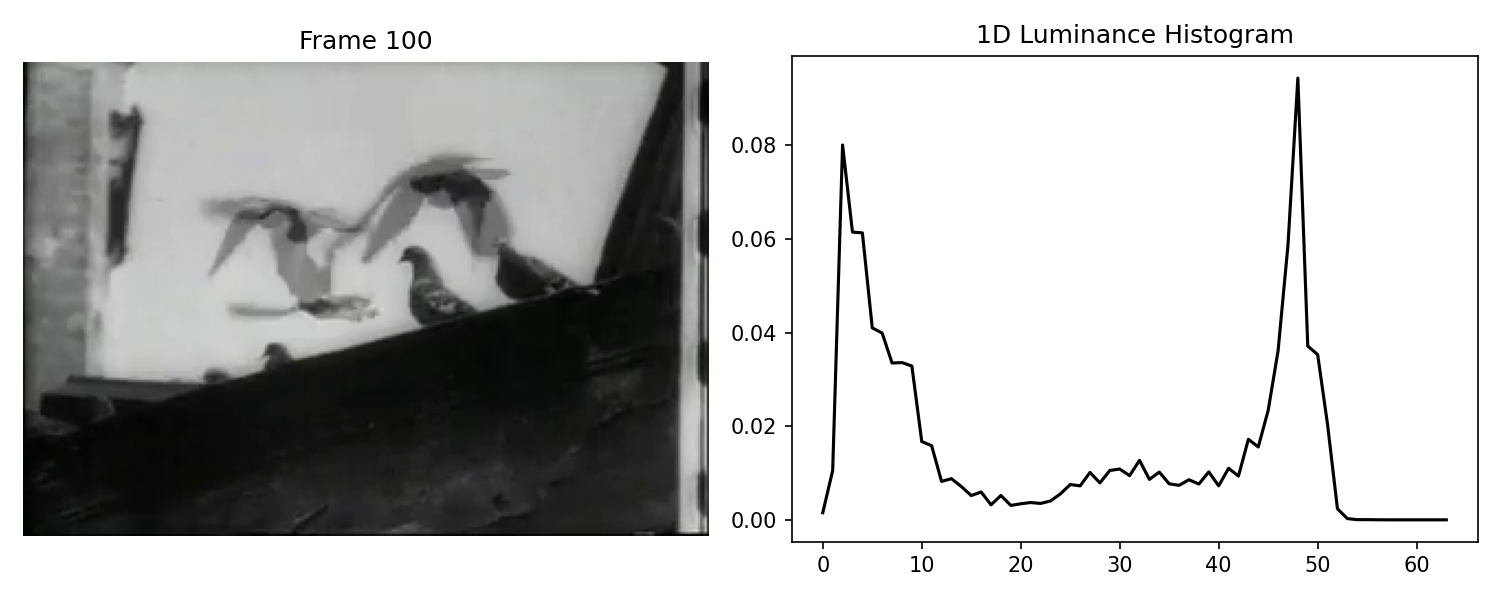
\includegraphics[width=0.9\textwidth]{Images/Extrait2-ManWithAMovieCamera_frame_100.png}
        \caption{Histogramme de luminance — Man With A Movie Camera (frame 100)}
    \end{figure}
    
    \begin{figure}[H]
        \centering
        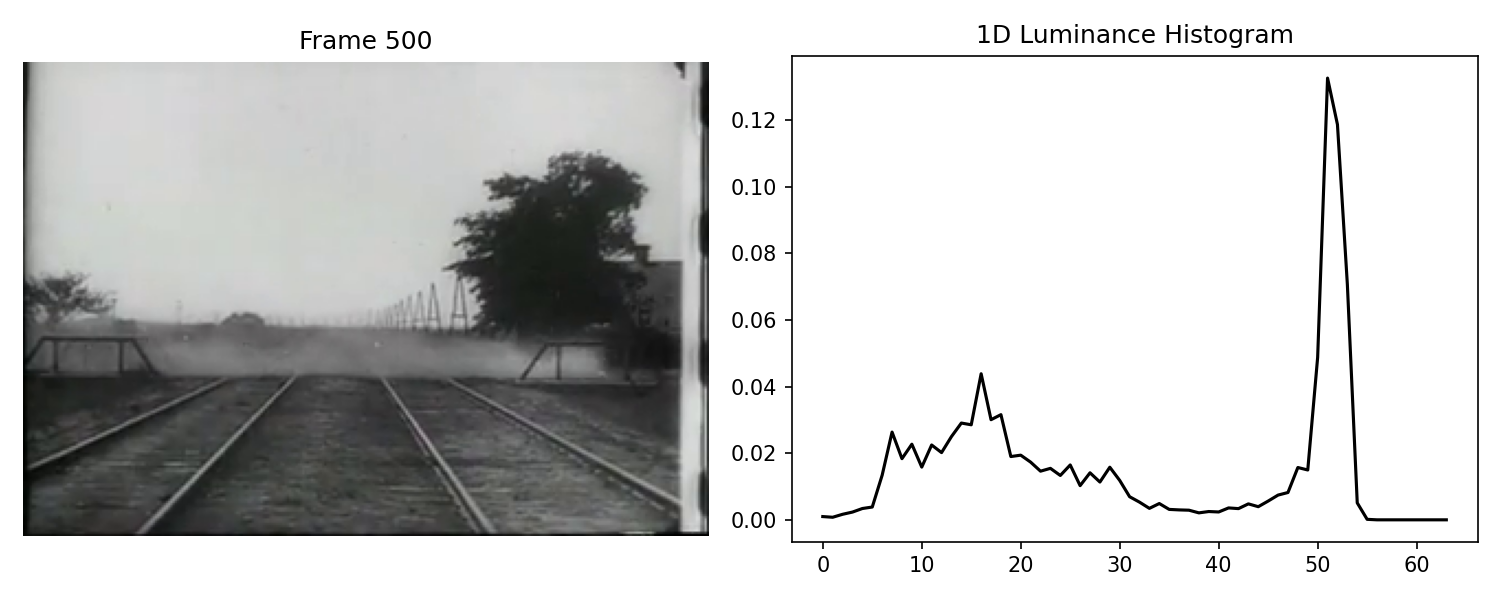
\includegraphics[width=0.9\textwidth]{Images/Extrait2-ManWithAMovieCamera_frame_500.png}
        \caption{Histogramme de luminance — Man With A Movie Camera (frame 500)}
    \end{figure}
    
    Les pics de l’histogramme correspondent aux régions sombres et claires dominantes dans l’image.
    
    % ==================================================
    % ENTRACTE
    % ==================================================
    
    \subsubsection*{Entracte}
    
    \begin{figure}[H]
        \centering
        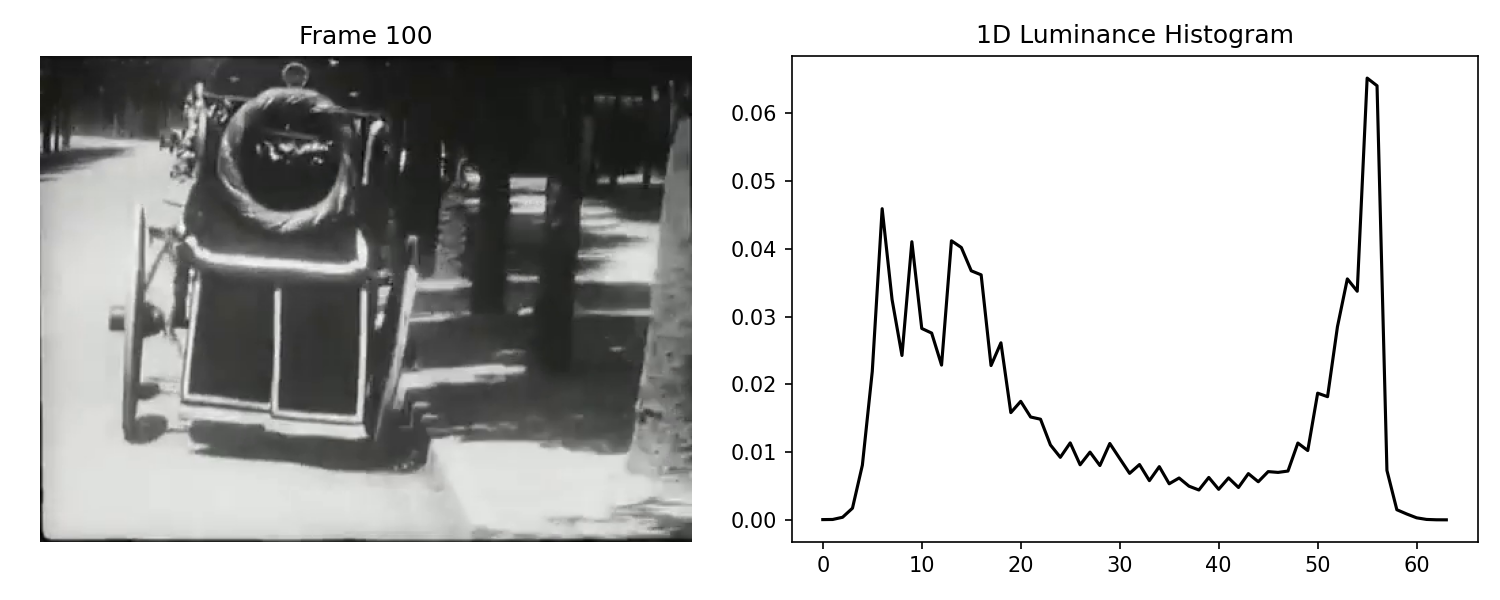
\includegraphics[width=0.9\textwidth]{Images/Extrait4-Entracte-Poursuite_Corbillard(358p)_frame_100.png}
        \caption{Histogramme de luminance — Entracte (frame 100)}
    \end{figure}
    
    \begin{figure}[H]
        \centering
        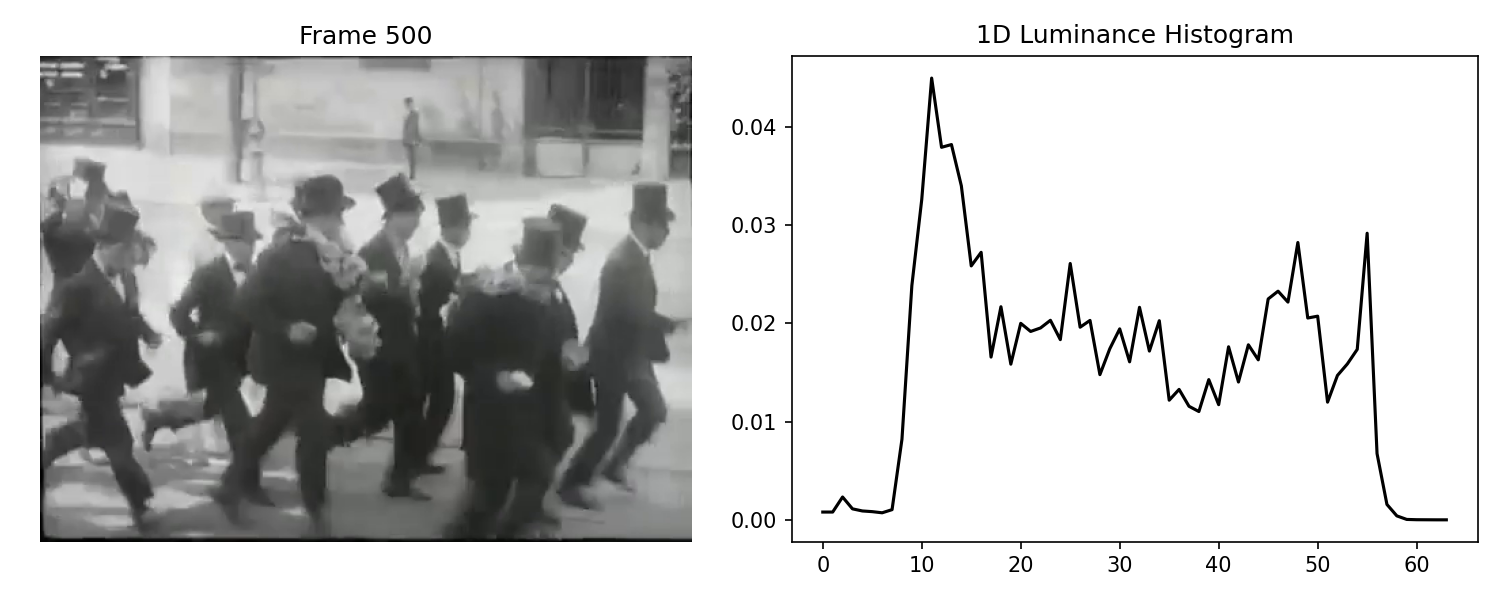
\includegraphics[width=0.9\textwidth]{Images/Extrait4-Entracte-Poursuite_Corbillard(358p)_frame_500.png}
        \caption{Histogramme de luminance — Entracte (frame 500)}
    \end{figure}
    
    Les variations de luminance permettent de distinguer les changements visuels importants malgré l’absence d’information chromatique.
    
    % ==================================================
    % HISTOGRAM DISTANCES
    % ==================================================
    
    \subsection*{Analyse temporelle des histogrammes}
    
    Afin d’analyser l’évolution temporelle des histogrammes, deux mesures de distance ont été utilisées :
    
    \begin{itemize}
        \item distance du Chi-carré
        \item distance de Bhattacharyya
    \end{itemize}
    
    Ces distances sont calculées entre les histogrammes de deux images consécutives.
    
    Une augmentation brutale de ces mesures peut indiquer un changement de plan.
    
    % ==================================================
    % GLOBAL RESULTS
    % ==================================================
    
    \begin{figure}[H]
        \centering
        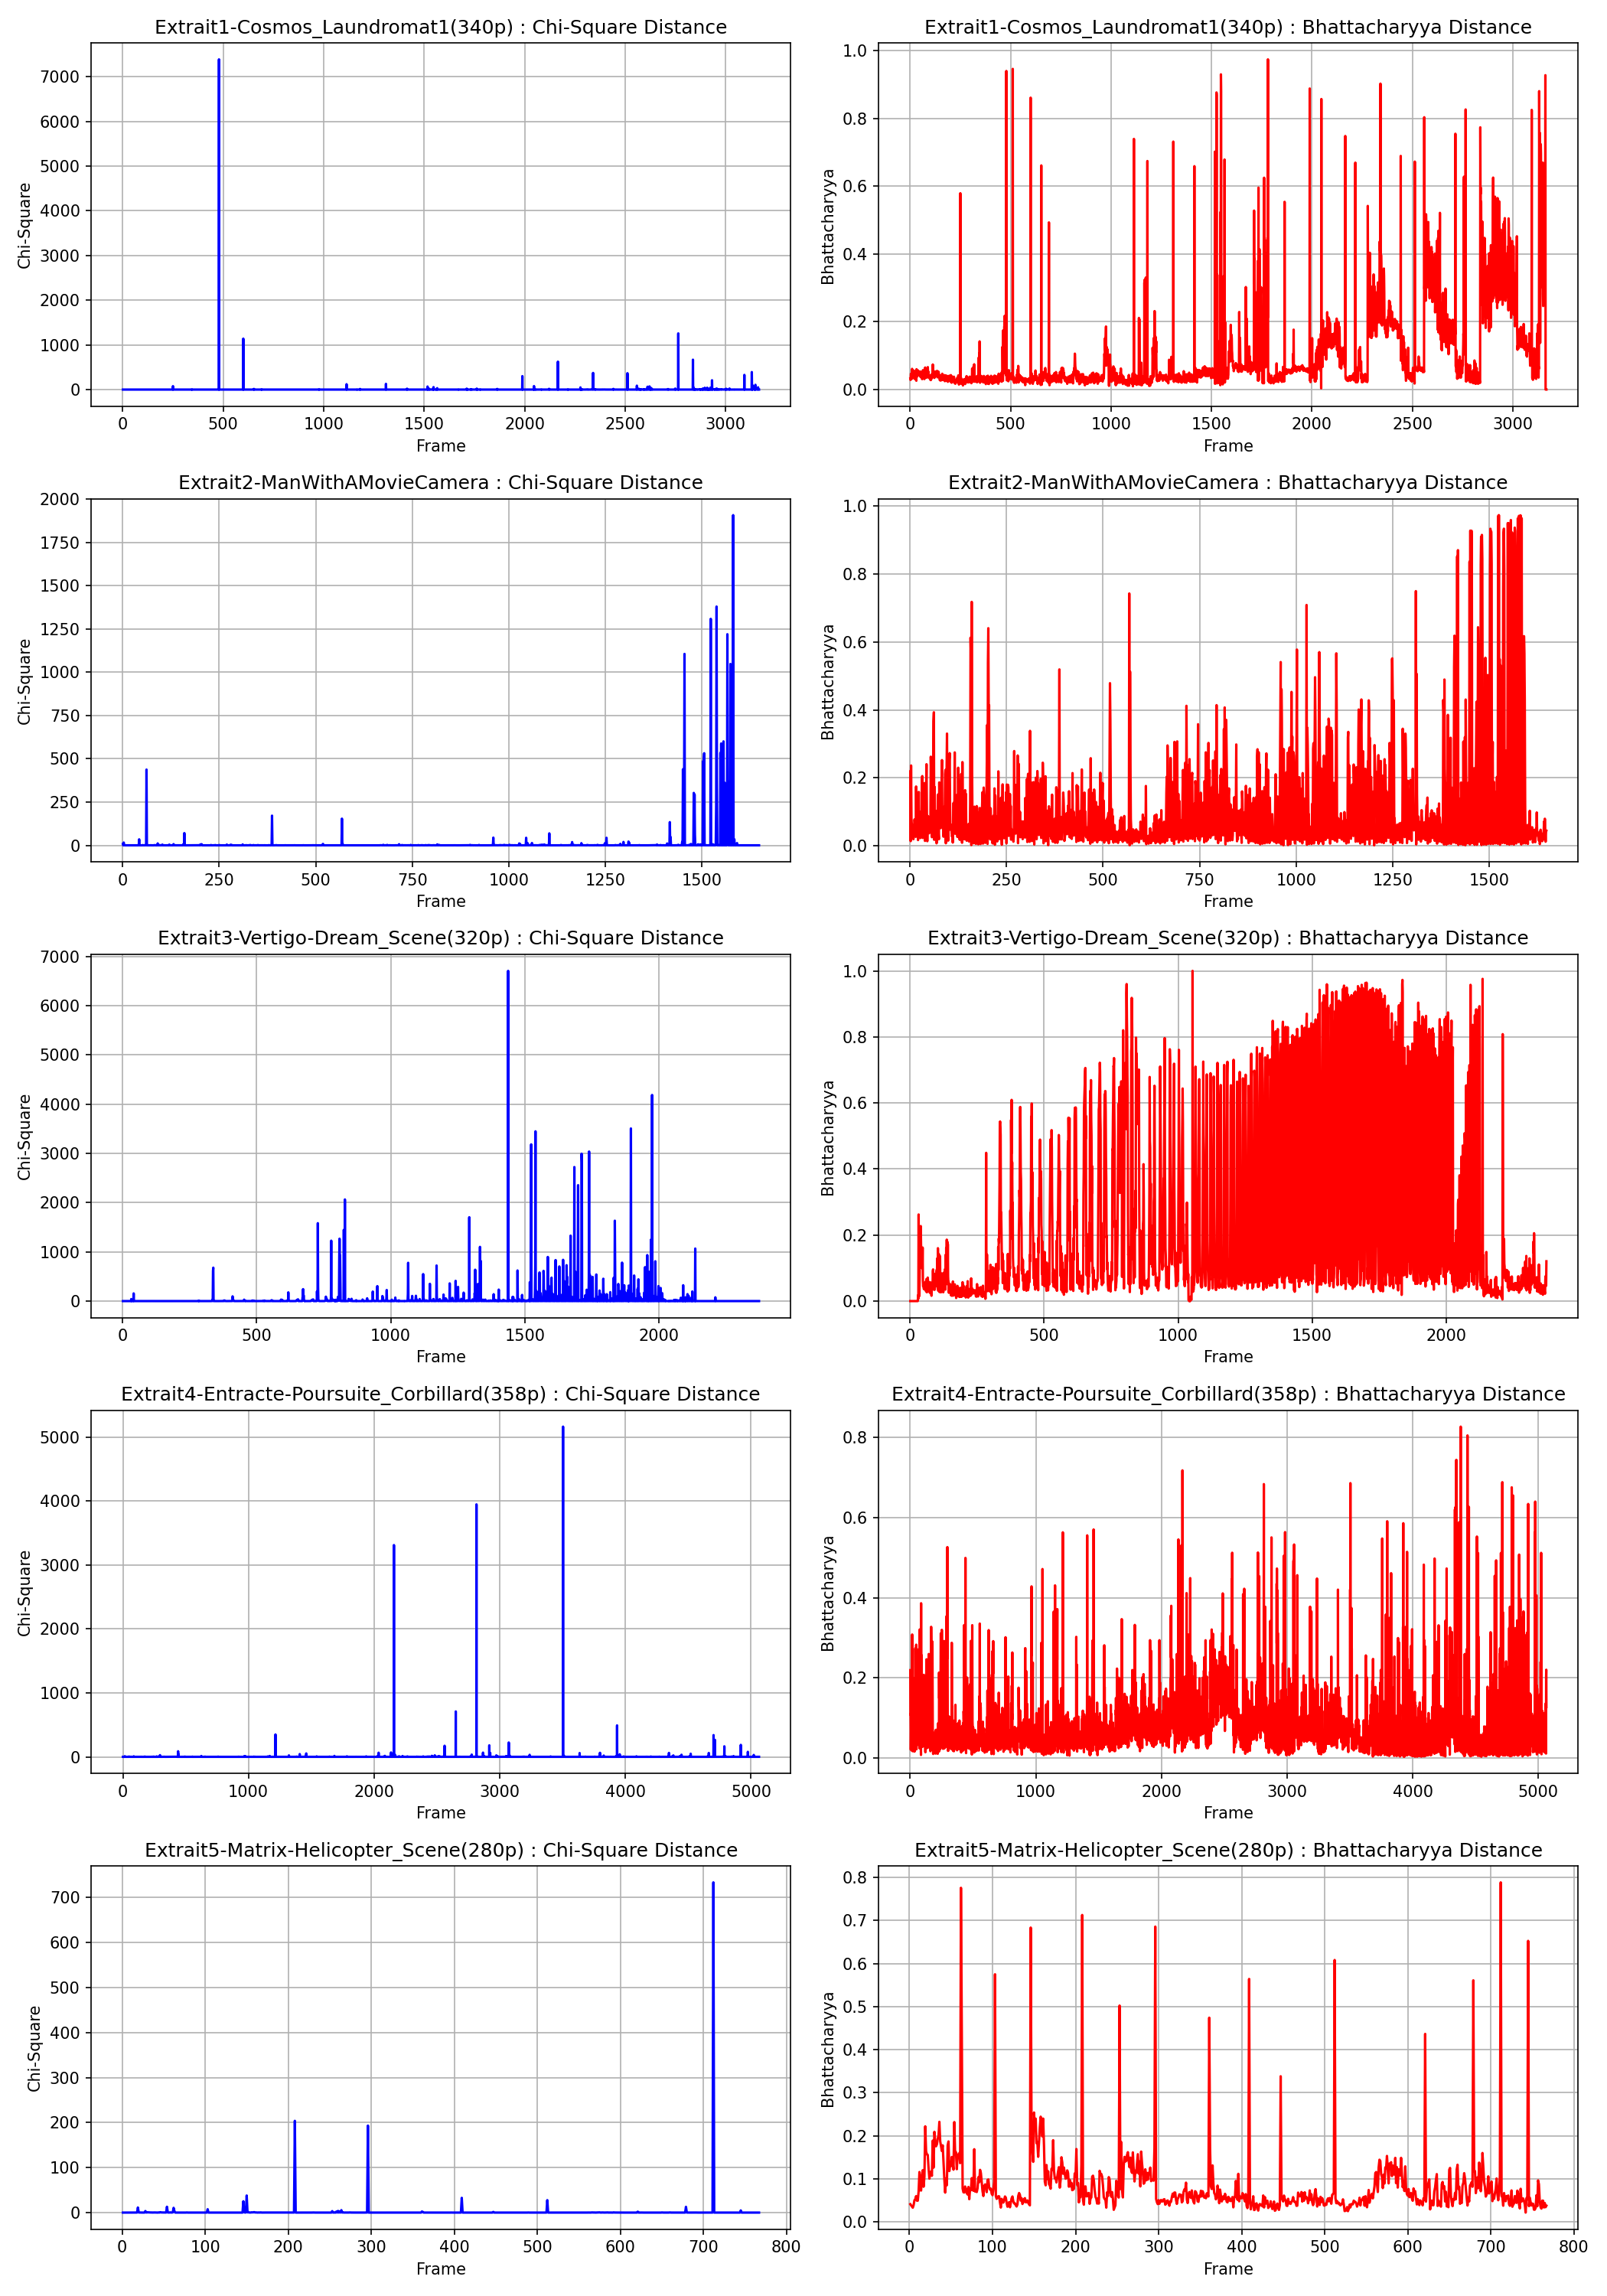
\includegraphics[width=\textwidth]{Images/q1_histogram_analysis.png}
        \caption{Évolution temporelle des distances entre histogrammes}
    \end{figure}
    
    On observe que :
    
    \begin{itemize}
        \item les distances restent généralement faibles à l’intérieur d’un même plan
        \item les changements de plan produisent des pics importants
        \item la distance du Chi-carré est  sensible aux variations brutales
    \end{itemize}
    
    % ==================================================
    % DISCUSSION
    % ==================================================
    
    \subsection*{Discussion}
    
    L’analyse des histogrammes chromatiques permet de caractériser efficacement le contenu global des images.
    
    Les changements de plan provoquent généralement une modification importante de la distribution des couleurs, ce qui se traduit par des pics dans les mesures de distance.
    
    Cependant, plusieurs difficultés apparaissent :
    
    \begin{itemize}
        \item mouvements rapides de caméra
        \item variations d’éclairage
        \item scènes fortement désaturées
        \item transitions progressives
    \end{itemize}
    
    Certaines séquences couleur possédant une dominante chromatique forte peuvent également produire des histogrammes très compacts.
    
    % ==================================================
    % CONCLUSION
    % ==================================================

    \subsection*{Conclusion}
    
    
    Cette première étude montre que les histogrammes YUV constituent une représentation pertinente pour l’analyse du contenu vidéo.
    
    Les distances entre histogrammes permettent de détecter de nombreuses transitions de plans de manière simple et efficace.
    
    Dans le cas des vidéos monochromes, l’utilisation d’un histogramme de luminance fournit une alternative adaptée.
    
    Ces observations serviront de base pour les méthodes plus avancées étudiées dans les parties suivantes du projet.
    
    \section*{Question II -- Histogrammes 2D du flot optique}
    
    Dans cette partie, nous étudions les propriétés statistiques du flot optique dense calculé entre deux images consécutives d’une vidéo.  
    L’objectif est d’analyser la distribution des vecteurs de mouvement afin d’identifier différents types de plans et d’observer les variations temporelles du mouvement dans les séquences vidéo.
    
    \vspace{0.3cm}
    
    Le flot optique dense est calculé à l’aide de la méthode de Farnebäck.  
    Pour chaque image, nous obtenons un champ de vecteurs :
    
    \[
    f(p) = (V_x(p), V_y(p))
    \]
    
    où :
    \begin{itemize}
        \item $V_x$ représente la composante horizontale du mouvement ;
        \item $V_y$ représente la composante verticale du mouvement.
    \end{itemize}
    
    À partir de ces composantes, nous construisons un histogramme bidimensionnel représentant la probabilité jointe des composantes $(V_x, V_y)$.
    
    \subsection*{Construction de l’histogramme 2D}
    
    Pour chaque paire d’images successives :
    \begin{enumerate}
        \item le flot optique dense est calculé ;
        \item les composantes $(V_x, V_y)$ sont extraites ;
        \item un histogramme 2D est construit ;
        \item l’histogramme est normalisé afin d’obtenir une distribution de probabilité.
    \end{enumerate}
    
    Afin d’éviter l’influence des valeurs extrêmes du flot optique, la plage de l’histogramme est définie à partir du 99\textsuperscript{e} percentile des amplitudes du mouvement.
    
    \vspace{0.3cm}
    
    Les histogrammes sont ensuite lissés par un filtre gaussien afin d’améliorer leur lisibilité visuelle.
    
    \subsection*{Visualisation des histogrammes du flot optique}
    
    Les figures suivantes montrent :
    \begin{itemize}
        \item l’image courante ;
        \item la visualisation du flot optique dense ;
        \item l’histogramme 2D des composantes $(V_x,V_y)$.
    \end{itemize}
    
    \subsubsection*{Vidéo 1}
    
    \begin{figure}[H]
        \centering
        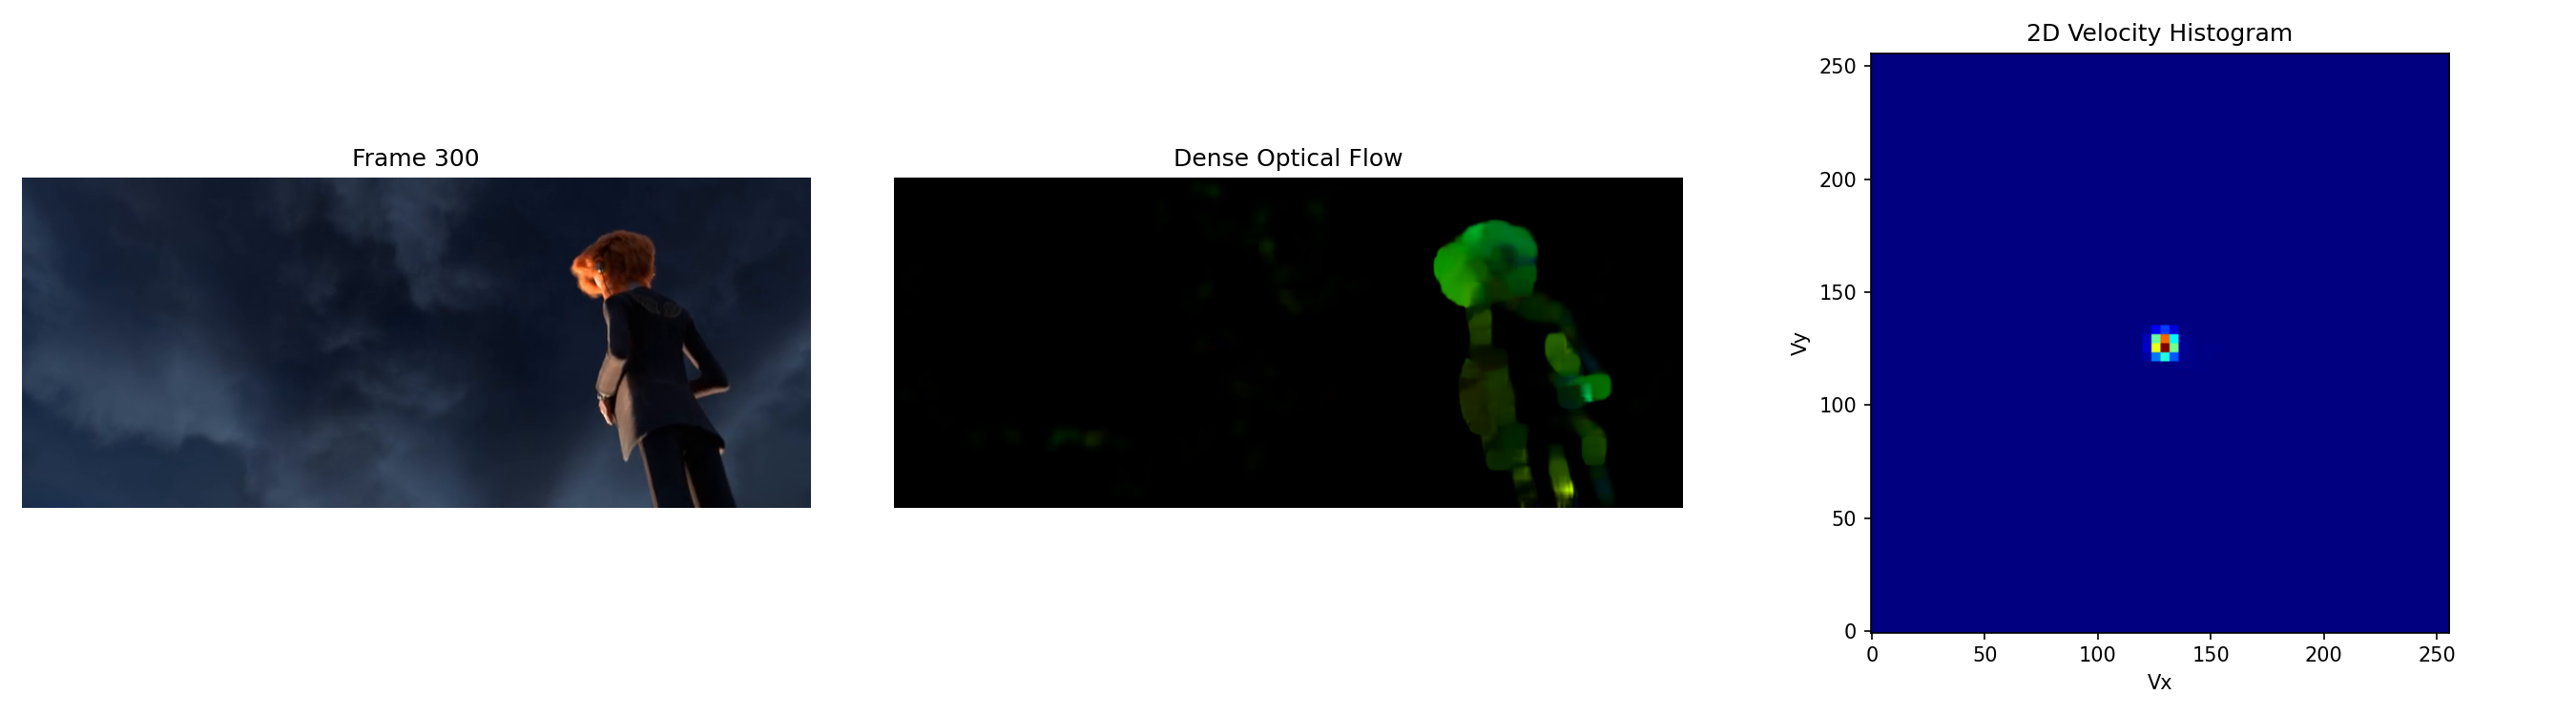
\includegraphics[width=\textwidth]{Images/Extrait1-Cosmos_Laundromat1(340p)_flow_histogram_300.png}
        \caption{Exemple d’histogramme 2D du flot optique pour la vidéo 1.}
    \end{figure}
    
    \subsubsection*{Vidéo 2}
    
    \begin{figure}[H]
        \centering
        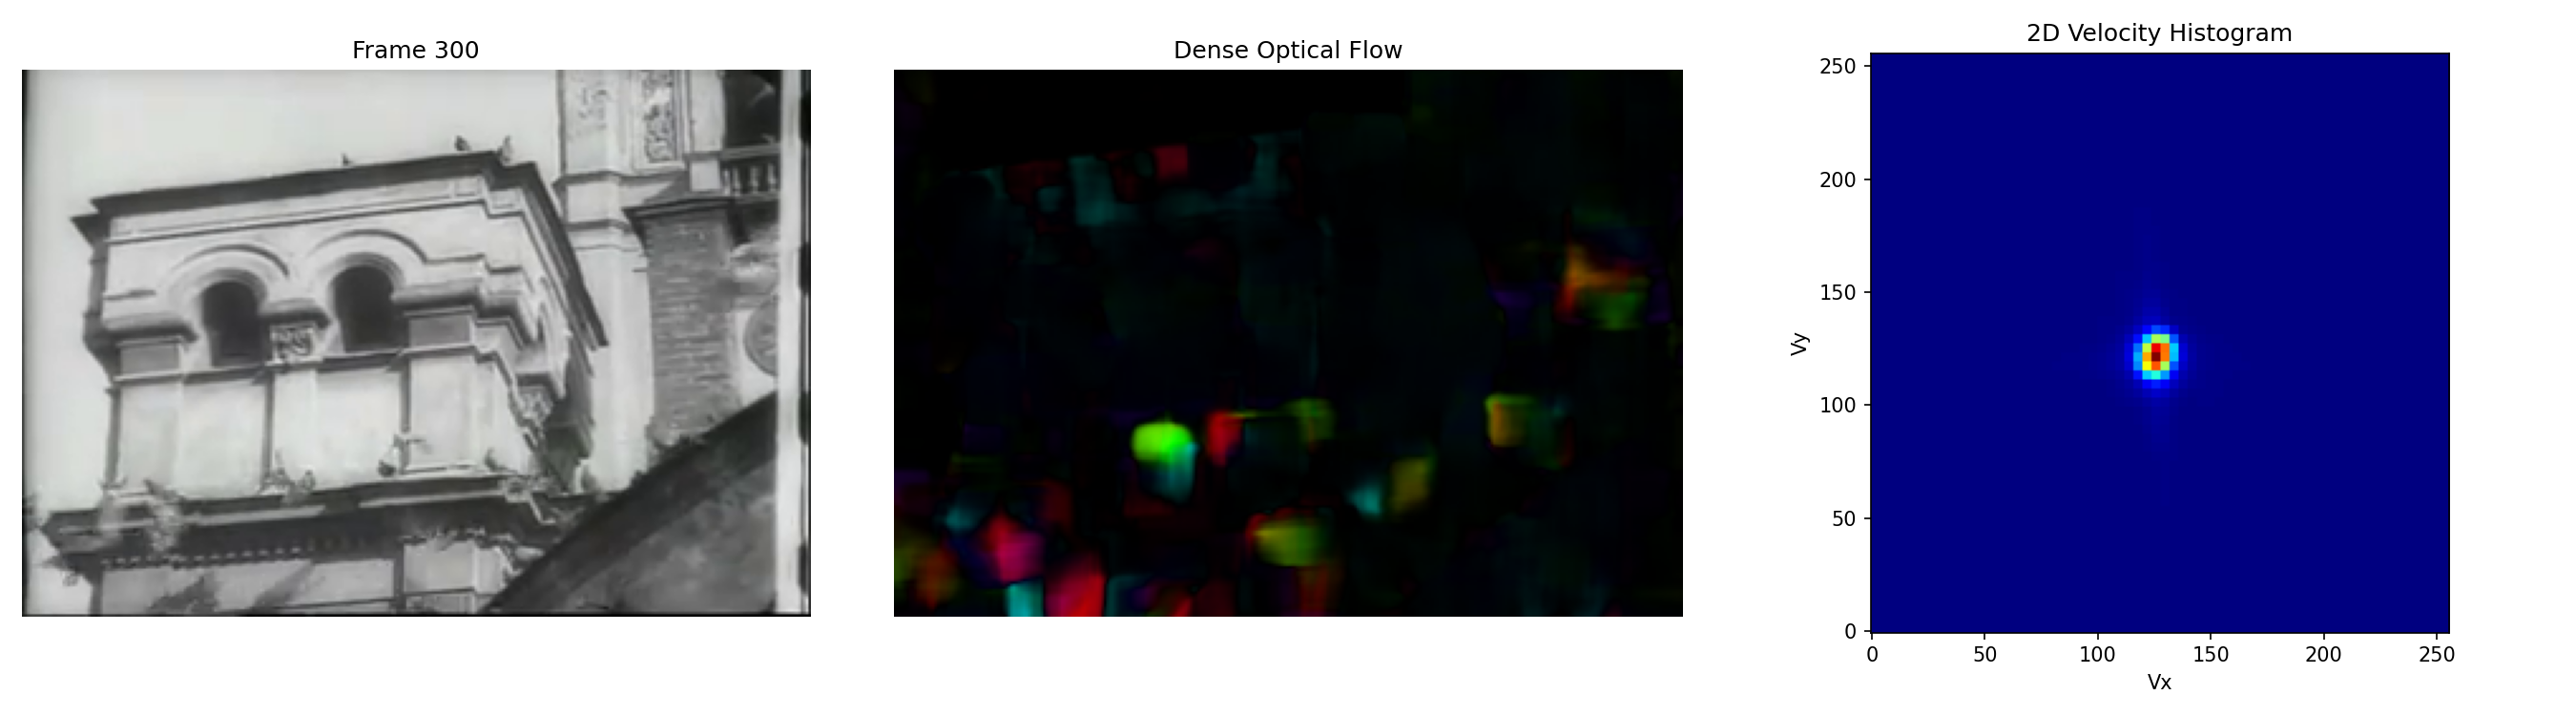
\includegraphics[width=\textwidth]{Images/Extrait2-ManWithAMovieCamera_flow_histogram_300.png}
        \caption{Exemple d’histogramme 2D du flot optique pour la vidéo 2.}
    \end{figure}
    
    \subsubsection*{Vidéo 3}
    
    \begin{figure}[H]
        \centering
        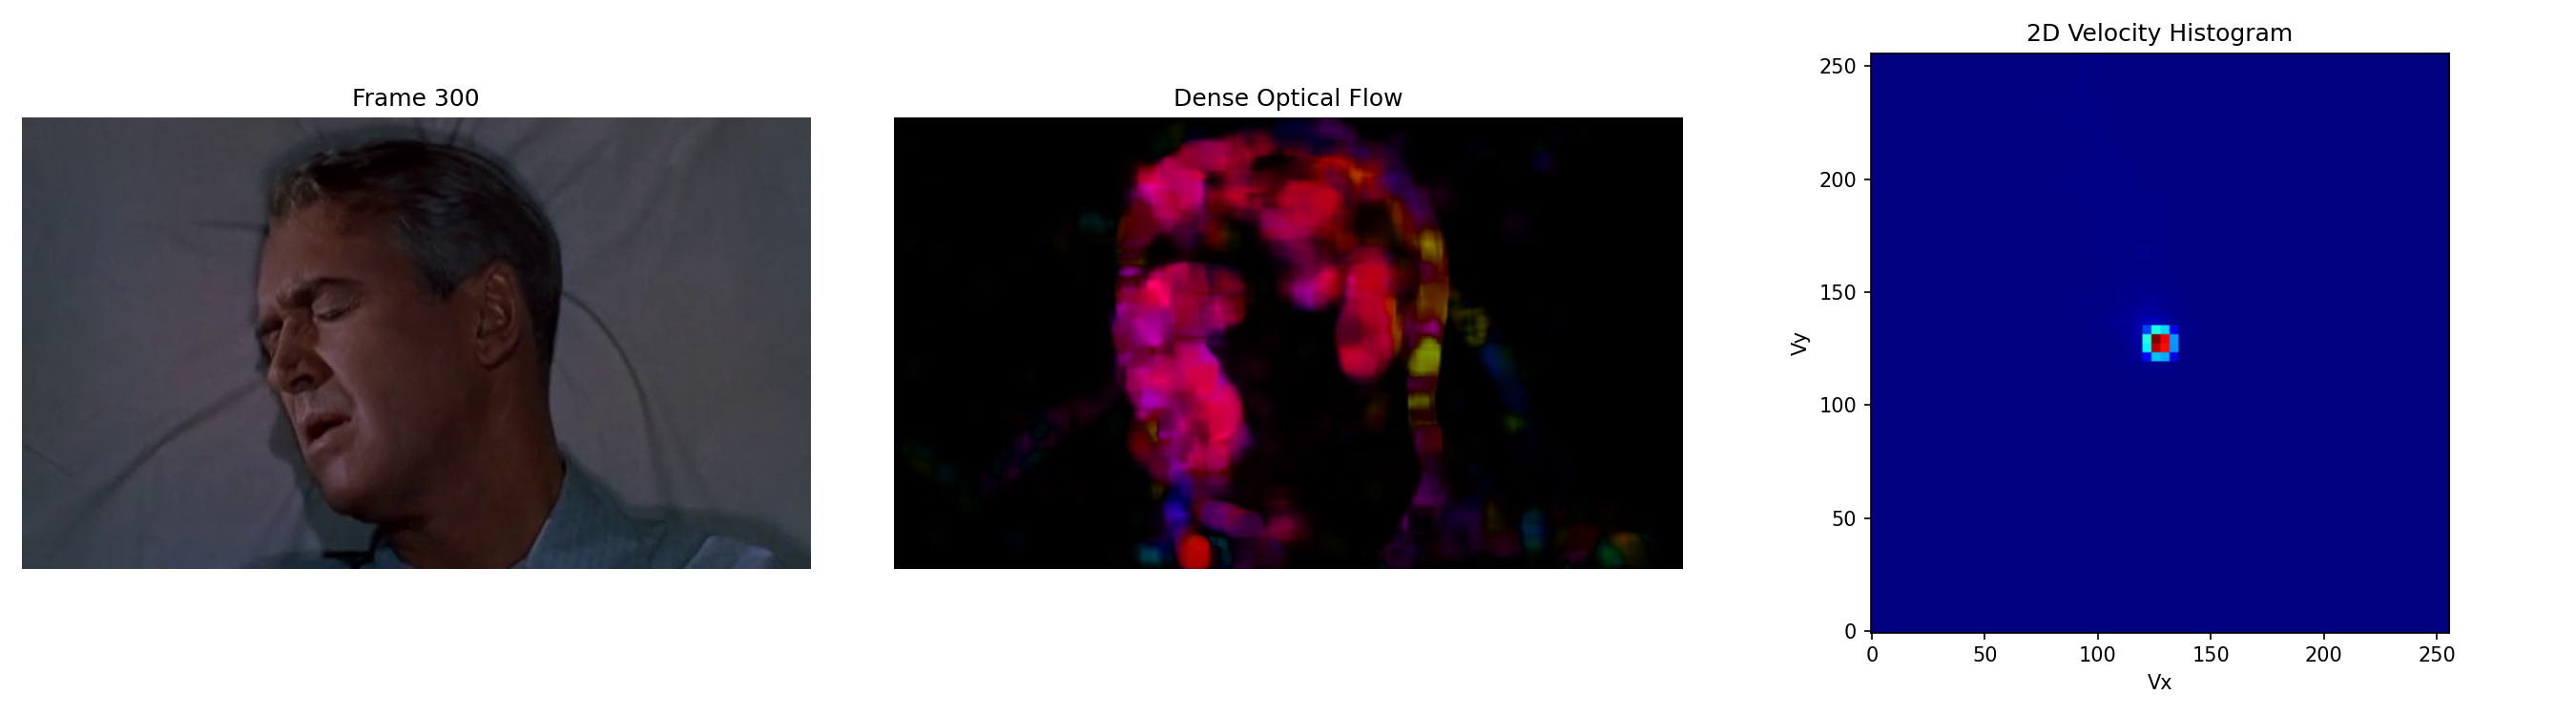
\includegraphics[width=\textwidth]{Images/Extrait3-Vertigo-Dream_Scene(320p)_flow_histogram_300.png}
        \caption{Exemple d’histogramme 2D du flot optique pour la vidéo 3.}
    \end{figure}
    
    \subsubsection*{Vidéo 4}
    
    \begin{figure}[H]
        \centering
        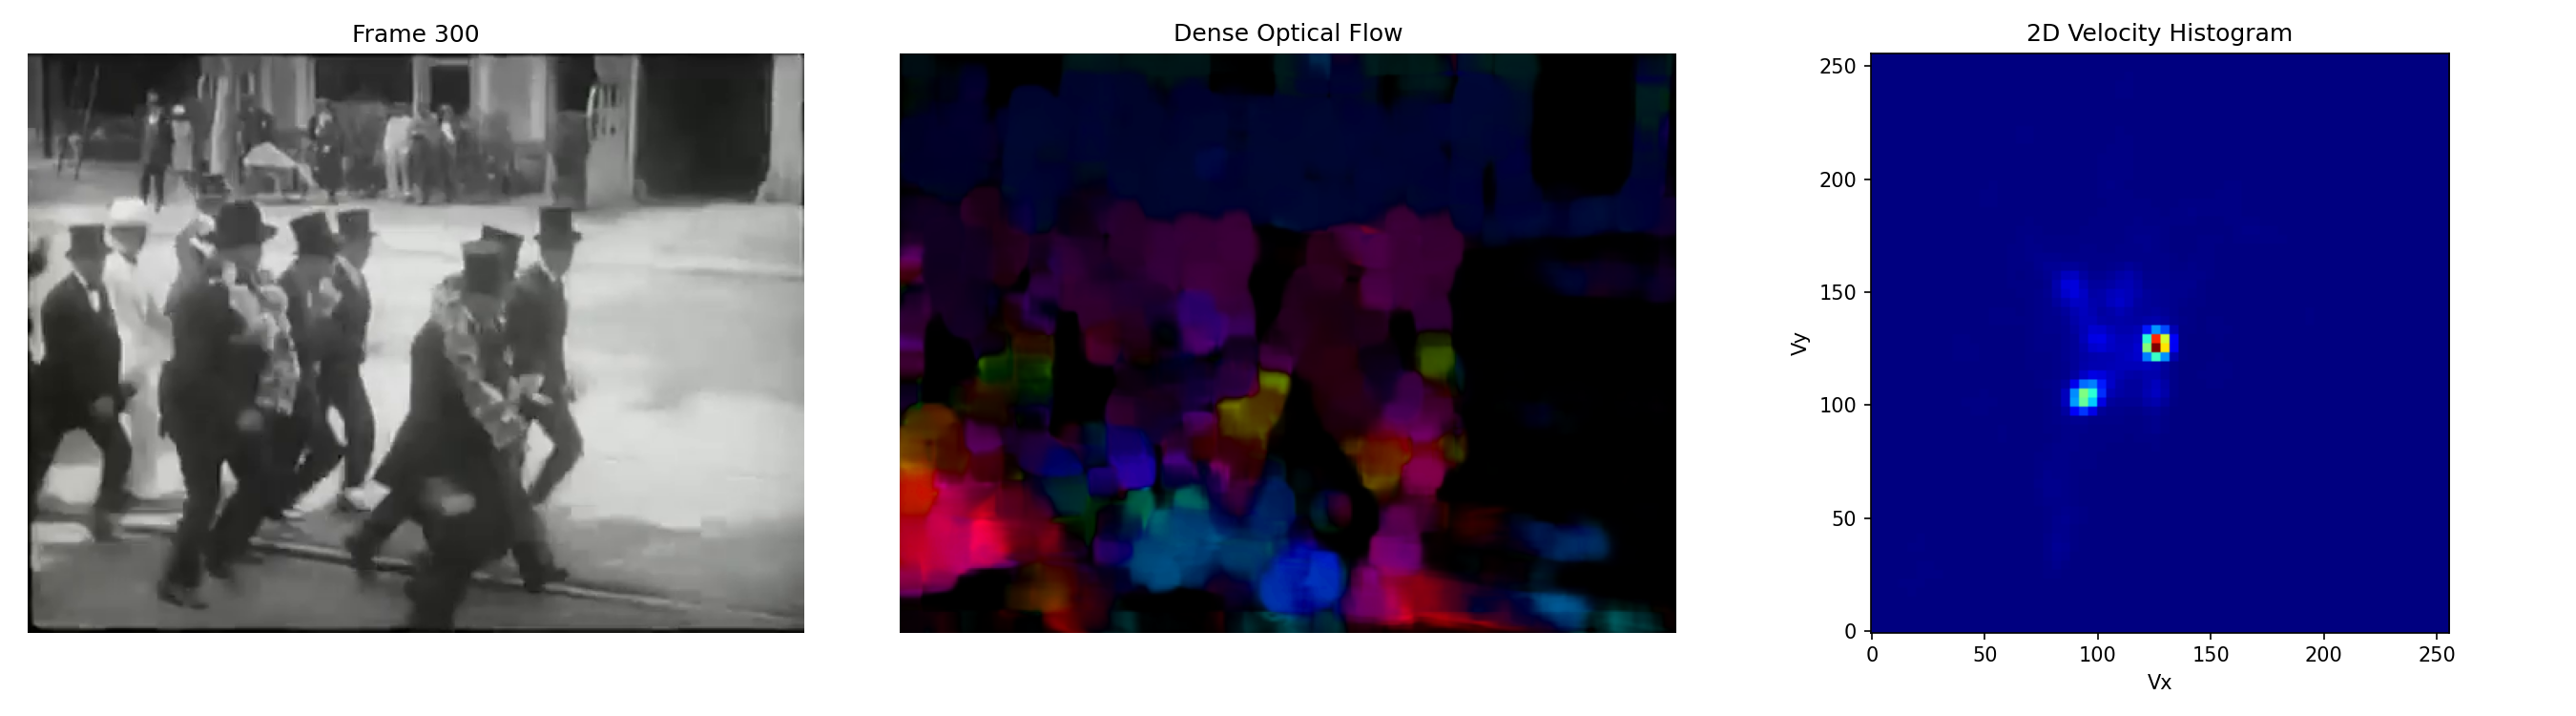
\includegraphics[width=\textwidth]{Images/Extrait4-Entracte-Poursuite_Corbillard(358p)_flow_histogram_300.png}
        \caption{Exemple d’histogramme 2D du flot optique pour la vidéo 4.}
    \end{figure}
    
    \subsubsection*{Vidéo 5}
    
    \begin{figure}[H]
        \centering
        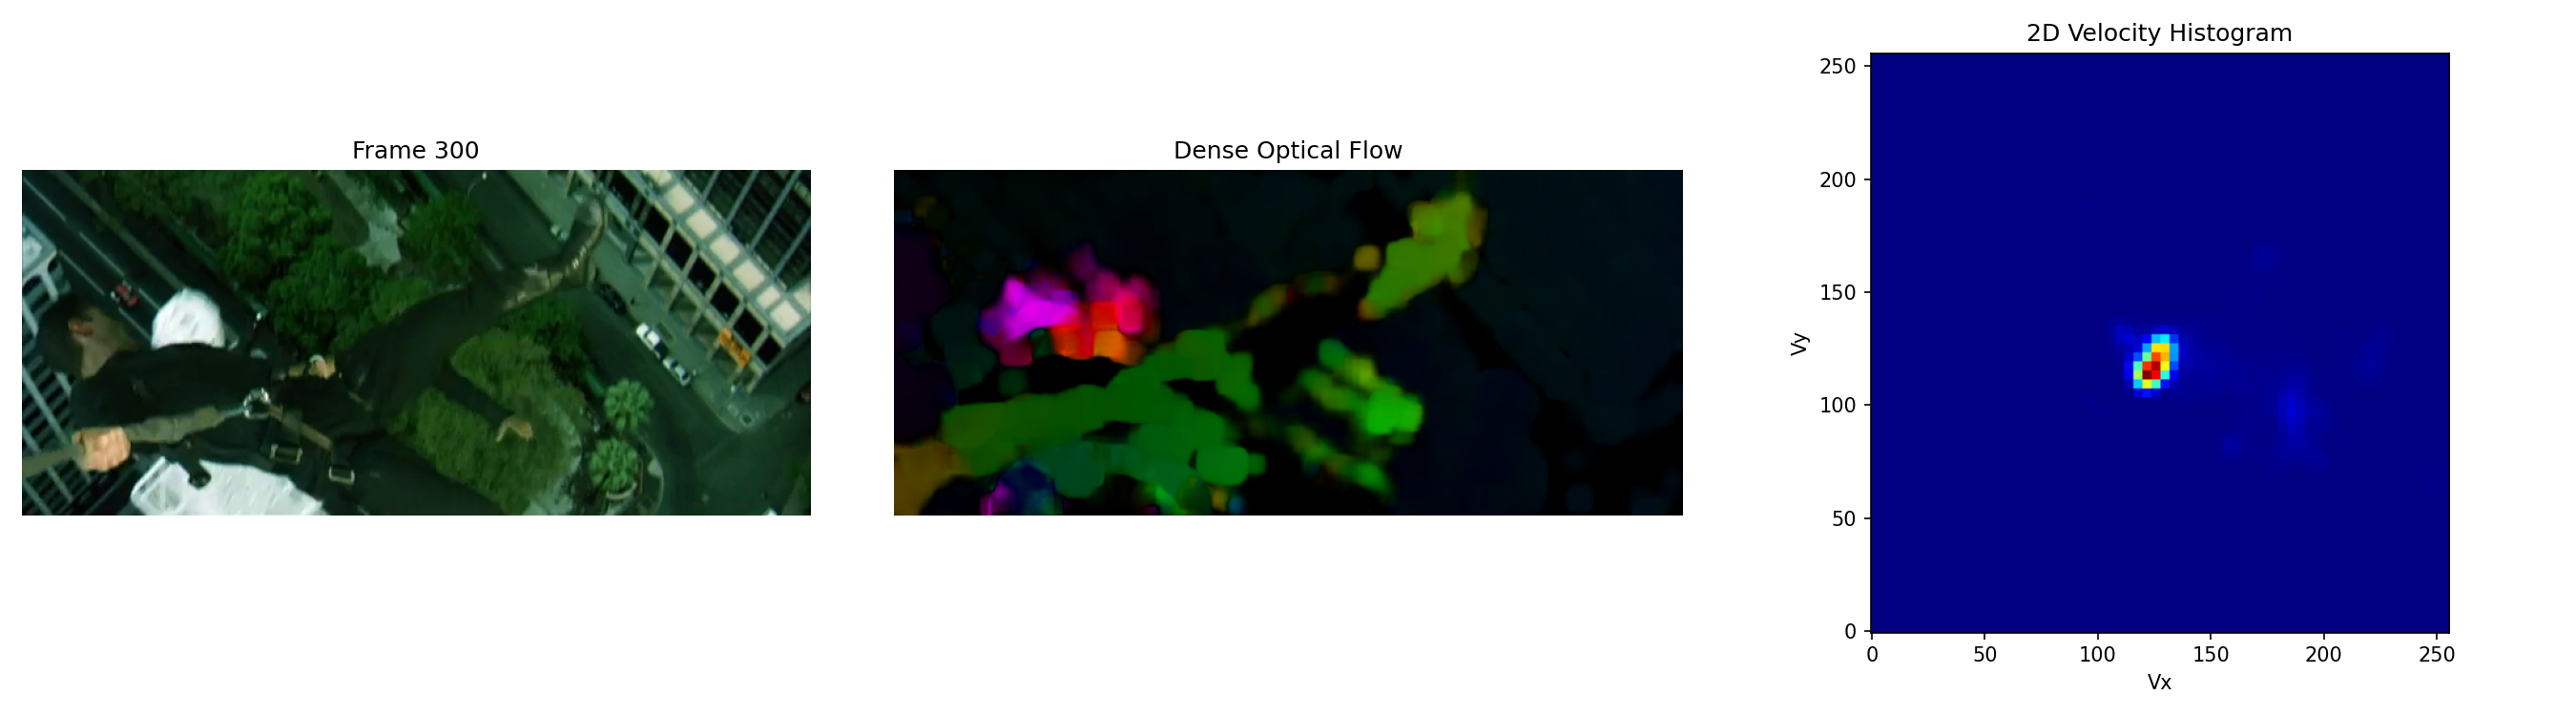
\includegraphics[width=\textwidth]{Images/Extrait5-Matrix-Helicopter_Scene(280p)_flow_histogram_300.png}
        \caption{Exemple d’histogramme 2D du flot optique pour la vidéo 5.}
    \end{figure}
    
    \subsection*{Analyse des histogrammes}
    
    Les histogrammes obtenus permettent d’observer plusieurs comportements caractéristiques du mouvement :
    
    \begin{itemize}
        \item lorsque le mouvement est faible, l’histogramme est fortement concentré autour de l’origine ;
        
        \item lors d’un déplacement global de caméra (travelling ou rotation), l’histogramme devient asymétrique et se déplace vers une direction dominante ;
        
        \item dans les scènes comportant plusieurs objets mobiles, l’histogramme devient plus dispersé et présente plusieurs zones d’énergie ;
        
        \item les scènes dynamiques génèrent généralement une distribution plus étendue des vitesses.
    \end{itemize}
    
    Ainsi, l’analyse de la forme et de la dispersion de l’histogramme permet d’obtenir des informations importantes sur la nature du mouvement présent dans la vidéo.
    
    \subsection*{Mesures temporelles}
    
    Afin d’étudier l’évolution temporelle du mouvement, plusieurs mesures statistiques ont été calculées :
    
    \begin{itemize}
        \item la magnitude moyenne du flot optique ;
        \item l’écart-type des amplitudes du mouvement ;
        \item l’entropie de l’histogramme 2D.
    \end{itemize}
    
    \begin{figure}[H]
        \centering
        
\includegraphics[width=\textwidth]{Images/q2_analysis.png}
        \caption{Évolution temporelle des statistiques du flot optique pour les différentes vidéos.}
    \end{figure}
    
    \subsection*{Interprétation des mesures}
    
    La magnitude moyenne permet d’évaluer l’intensité globale du mouvement dans la scène.  
    Les pics observés correspondent généralement à des mouvements importants de caméra ou à des scènes très dynamiques.
    
    \vspace{0.3cm}
    
    L’écart-type mesure la dispersion des vitesses et permet d’identifier les scènes comportant plusieurs mouvements indépendants.
    
    \vspace{0.3cm}
    
    Enfin, l’entropie de l’histogramme représente la complexité du mouvement :
    \begin{itemize}
        \item une faible entropie correspond à un mouvement cohérent et organisé ;
        \item une forte entropie indique une distribution plus complexe des vecteurs de mouvement.
    \end{itemize}
    
    Ces mesures peuvent être utilisées pour détecter certains changements de plan ou pour différencier plusieurs types de mouvements cinématographiques.
    
    \subsection*{Identification du type de plan}
    
    L’analyse des histogrammes du flot optique permet d’identifier plusieurs types de plans :
    
    \begin{itemize}
        \item les plans statiques produisent des histogrammes concentrés autour de zéro ;
        
        \item les travellings horizontaux produisent une distribution décalée selon l’axe $V_x$ ;
        
        \item les mouvements verticaux produisent une distribution orientée selon $V_y$ ;
        
        \item les scènes complexes contenant plusieurs objets mobiles génèrent des histogrammes plus dispersés.
    \end{itemize}
    
    Ainsi, la structure de l’histogramme constitue une représentation compacte et informative du mouvement présent dans la vidéo.
    
    \subsection*{Conclusion}
    
    Cette étude montre que les histogrammes 2D du flot optique constituent une représentation efficace pour analyser le mouvement dans une séquence vidéo.
    
    Les différentes mesures statistiques calculées permettent d’observer les variations temporelles du mouvement et fournissent des indices utiles pour l’identification des types de plans ainsi que pour la détection de changements importants dans la dynamique de la scène.
        

    \section*{Question III -- Détection des changements de plans à partir des images résiduelles}
    
    Dans cette partie, nous exploitons le flot optique afin de prédire les images successives d’une séquence vidéo, puis d’analyser les erreurs de prédiction afin de détecter les changements de plans.
    
    \vspace{0.3cm}
    
    À partir du flot optique dense calculé entre deux images successives, nous construisons une image prédite :
    
    \[
    \hat{I}_t(p)=I_{t-1}(p+f_{t-1\rightarrow t}(p))
    \]
    
    où :
    \begin{itemize}
        \item $I_{t-1}$ représente l’image précédente ;
        \item $f_{t-1\rightarrow t}(p)$ correspond au vecteur du flot optique au pixel $p$ ;
        \item $\hat{I}_t$ est l’image prédite.
    \end{itemize}
    
    L’idée principale est qu’en l’absence de changement de plan, le flot optique permet de reconstruire correctement l’image suivante.  
    En revanche, lors d’un changement brutal de scène, la prédiction devient incorrecte et l’erreur résiduelle augmente fortement.
    
    \subsection*{Calcul de l’image résiduelle}
    
    L’image résiduelle est définie par :
    
    \[
    R_t = I_t - \hat{I}_t
    \]
    
    Dans notre implémentation, l’image prédite est calculée à partir d’un recalage de l’image précédente utilisant le flot optique dense de Farnebäck.
    
    \vspace{0.3cm}
    
    Les figures suivantes montrent :
    \begin{itemize}
        \item l’image courante ;
        \item l’image prédite ;
        \item l’image résiduelle correspondante.
    \end{itemize}
    
    \subsection*{Exemples d’images résiduelles}
    
    \subsubsection*{Vidéo 1 -- Cosmos Laundromat}
    
    \begin{figure}[H]
        \centering
        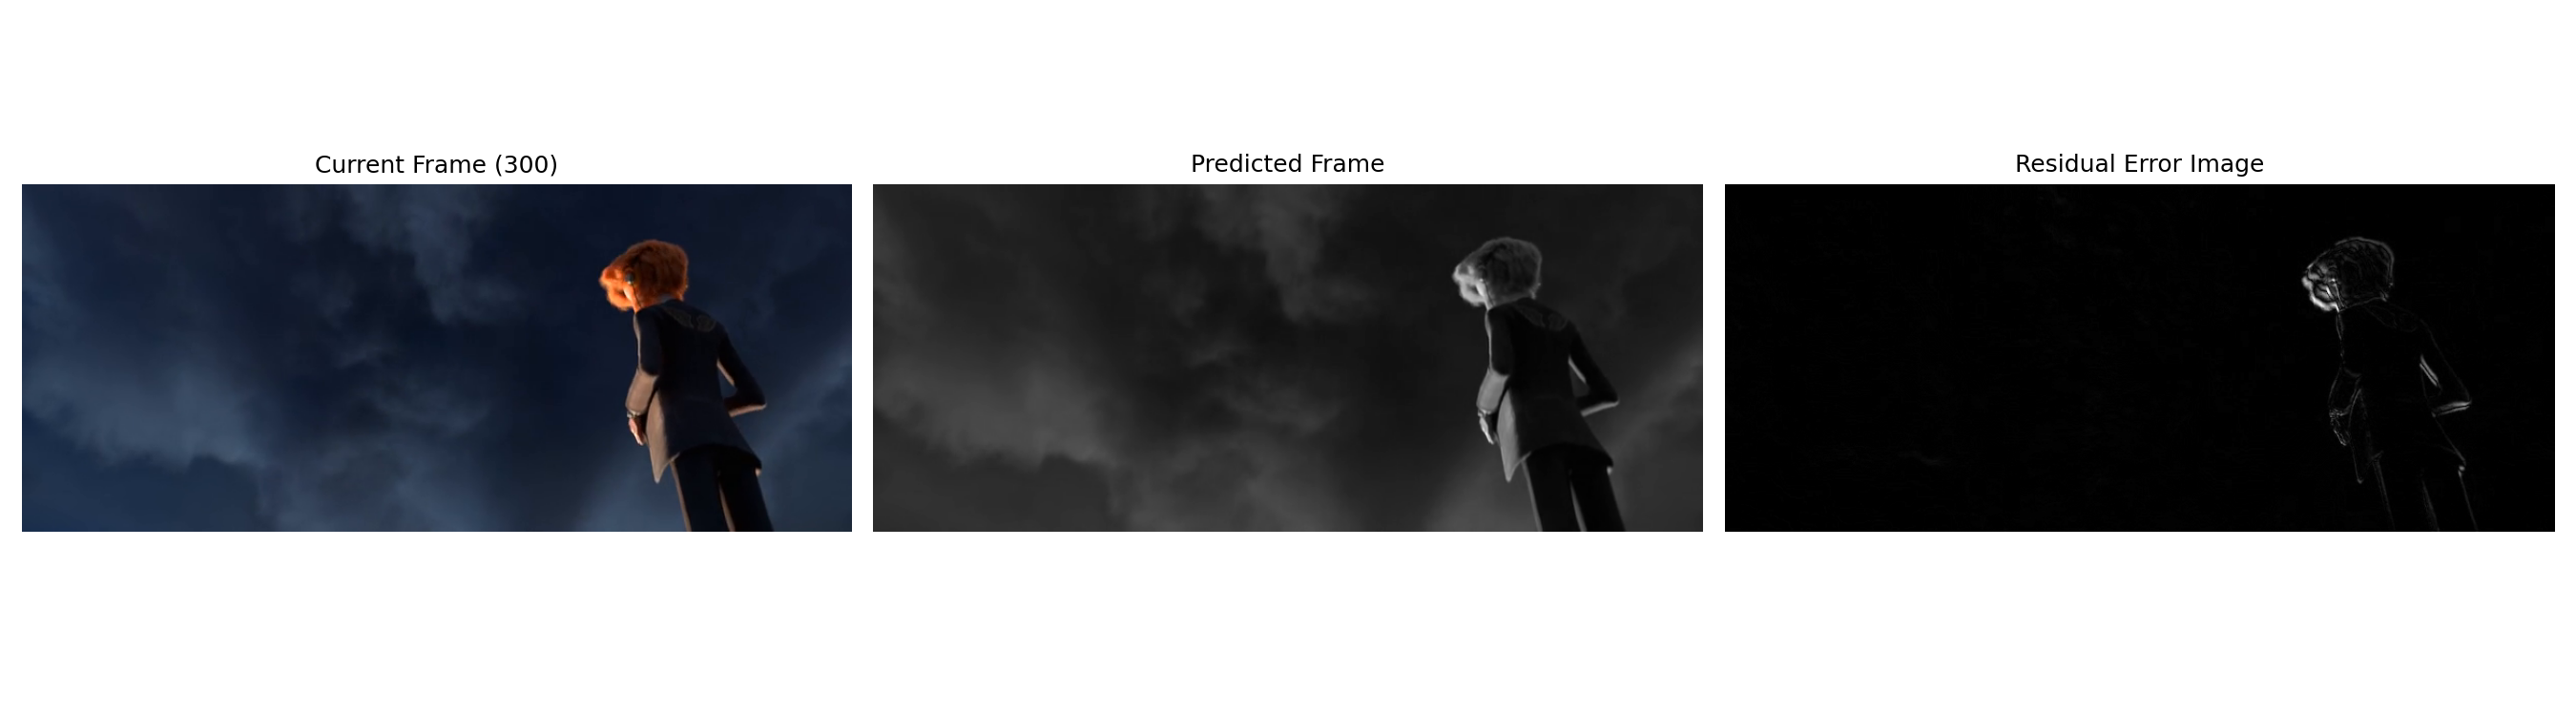
\includegraphics[width=\textwidth]{Images/q3_cosmos_residual.png}
        \caption{Exemple d’image résiduelle pour la vidéo Cosmos Laundromat.}
    \end{figure}
    
    Les changements de plans produisent des résidus importants et fortement structurés.  
    La majorité des transitions ont été correctement détectées dans cette séquence.
    
    \vspace{0.3cm}
    
    Quelques faux négatifs subsistent cependant lors de transitions présentant des couleurs ou des mouvements similaires entre deux plans consécutifs.
    
    \subsubsection*{Vidéo 2 -- Man With A Movie Camera}
    
    \begin{figure}[H]
        \centering
        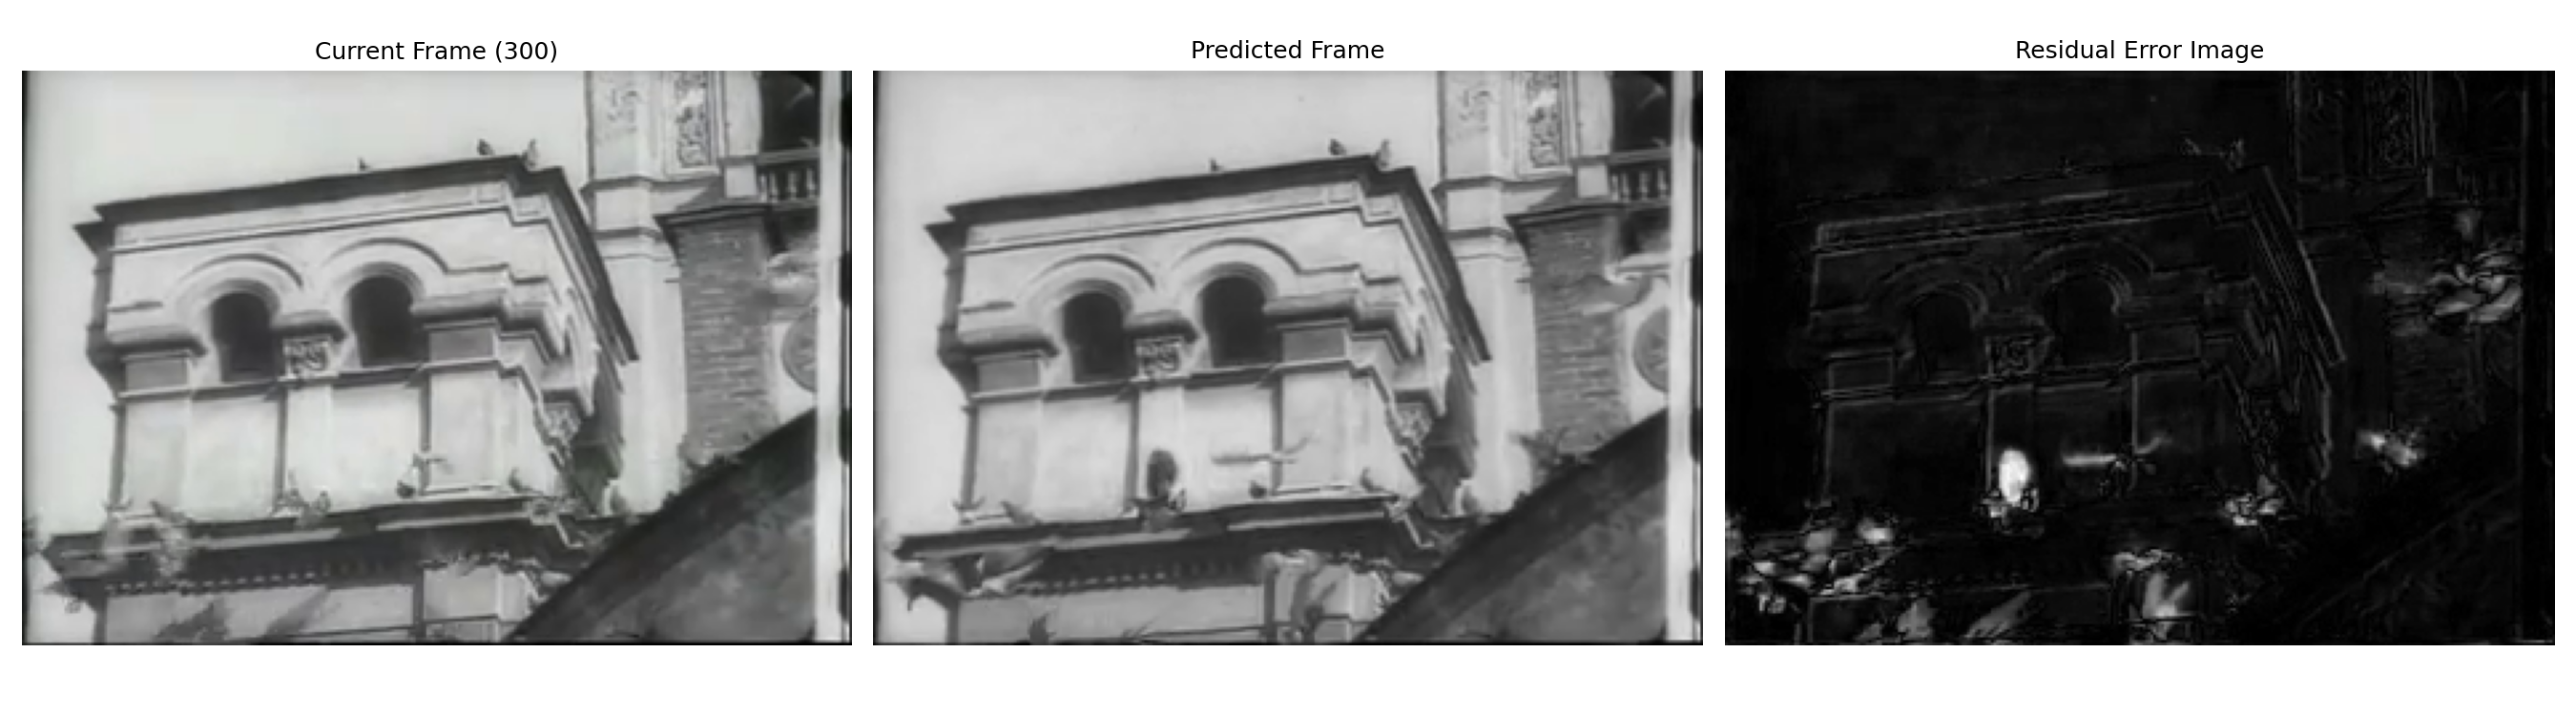
\includegraphics[width=\textwidth]{Images/q3_moviecamera_residual.png}
        \caption{Exemple d’image résiduelle pour la vidéo monochrome.}
    \end{figure}
    
    Dans les vidéos monochromes, la détection devient plus difficile car l’information chromatique est absente.  
    Les histogrammes de niveaux de gris sont moins discriminants et certains faux positifs apparaissent à cause du bruit et des variations de contraste.
    
    \subsubsection*{Vidéo 3 -- Vertigo}
    
    \begin{figure}[H]
        \centering
        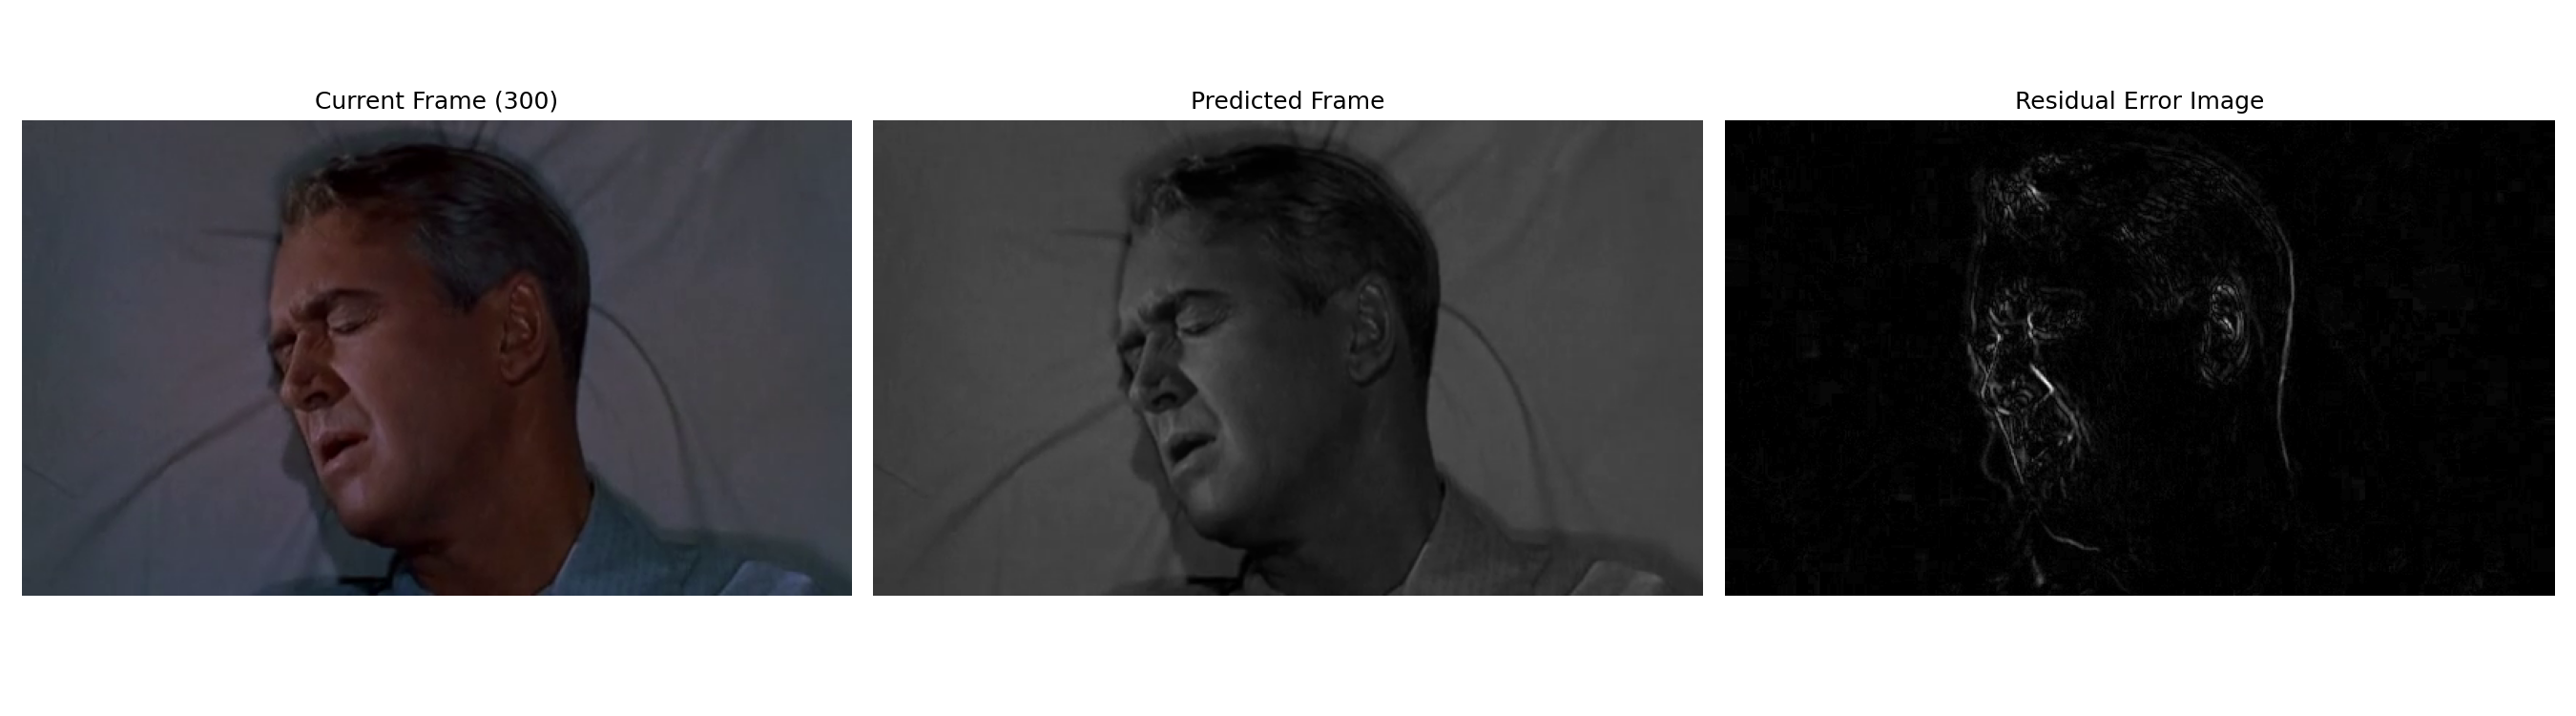
\includegraphics[width=\textwidth]{Images/q3_vertigo_residual.png}
        \caption{Exemple d’image résiduelle pour la vidéo Vertigo.}
    \end{figure}
    
    Cette vidéo contient de nombreuses variations lumineuses et changements rapides de couleurs.  
    Le détecteur produit alors plusieurs faux positifs, notamment lors des effets de clignotement et des changements brusques d’éclairage.
    
    \vspace{0.3cm}
    
    Ces phénomènes augmentent fortement l’entropie des résidus sans correspondre à de véritables changements de plans.
    
    \subsubsection*{Vidéo 4 -- Entracte}
    
    \begin{figure}[H]
        \centering
        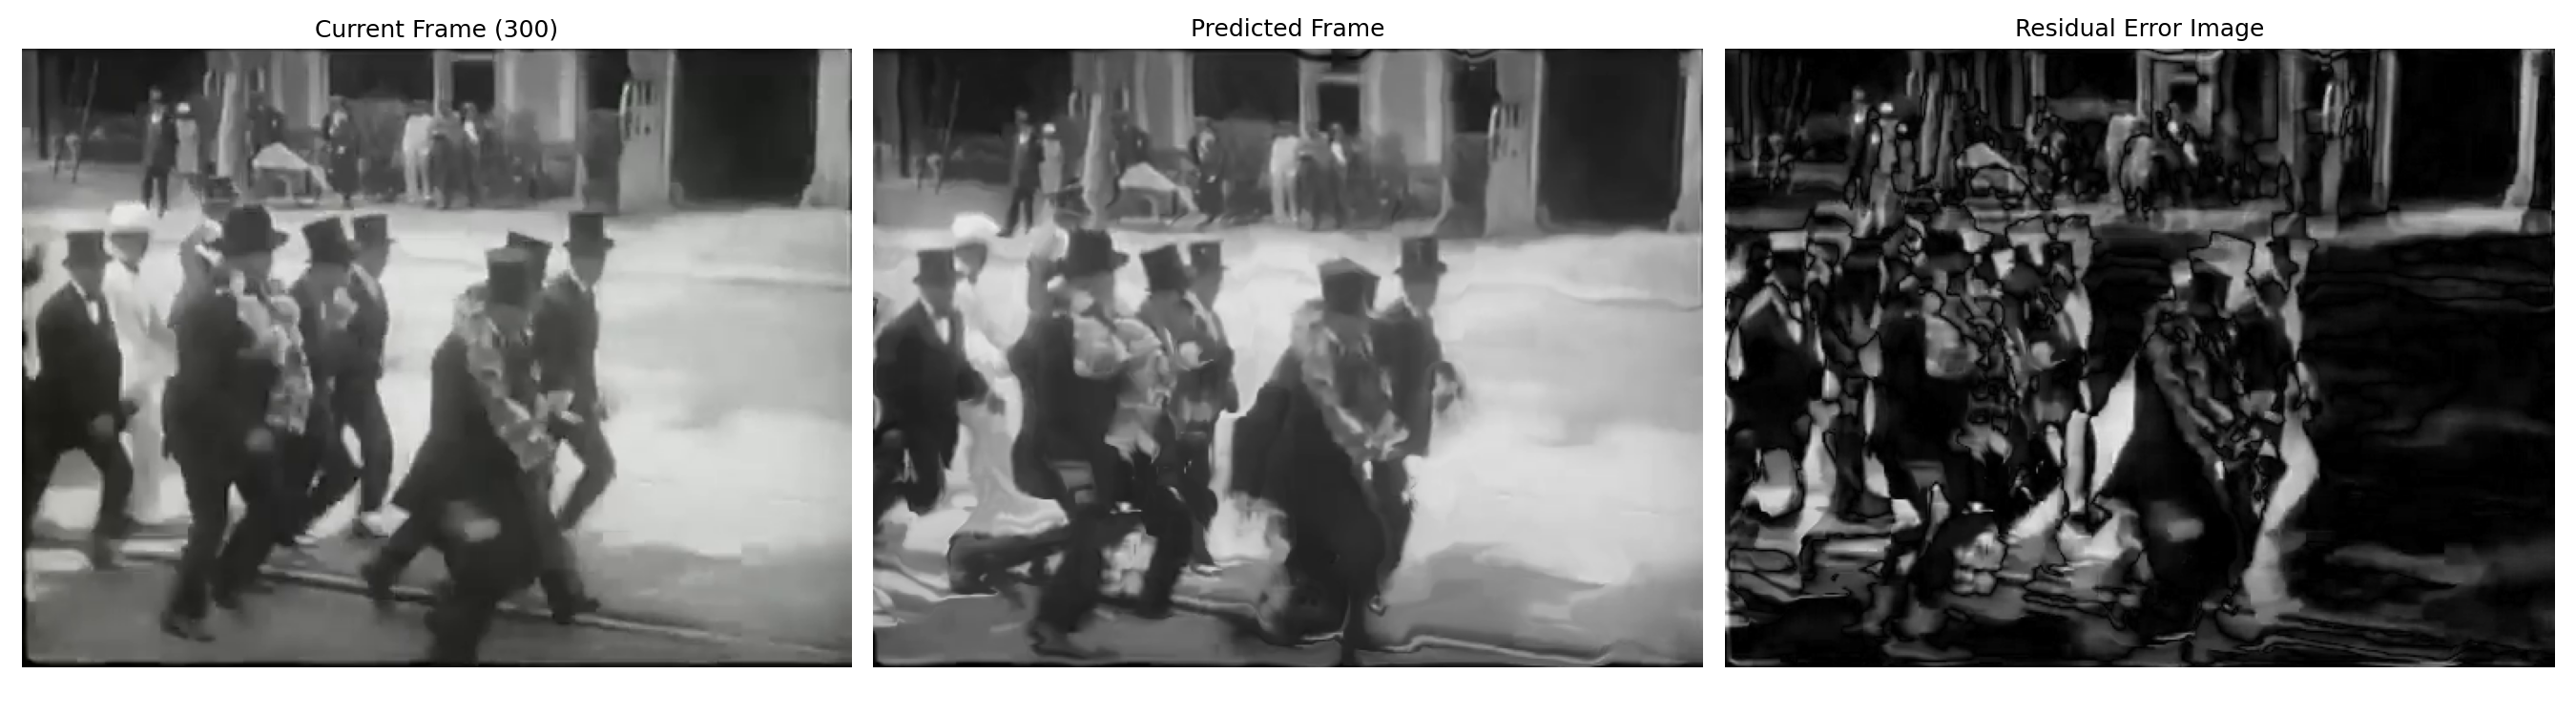
\includegraphics[width=\textwidth]{Images/q3_entracte_residual.png}
        \caption{Exemple d’image résiduelle pour la vidéo Entracte.}
    \end{figure}
    
    Les résultats obtenus sont globalement satisfaisants malgré quelques faux positifs et certaines transitions non détectées.
    
    \vspace{0.3cm}
    
    Les mouvements rapides et les fluctuations d’intensité caractéristiques des anciennes vidéos compliquent la prédiction par flot optique.
    
    \subsubsection*{Vidéo 5 -- Matrix}
    
    \begin{figure}[H]
        \centering
        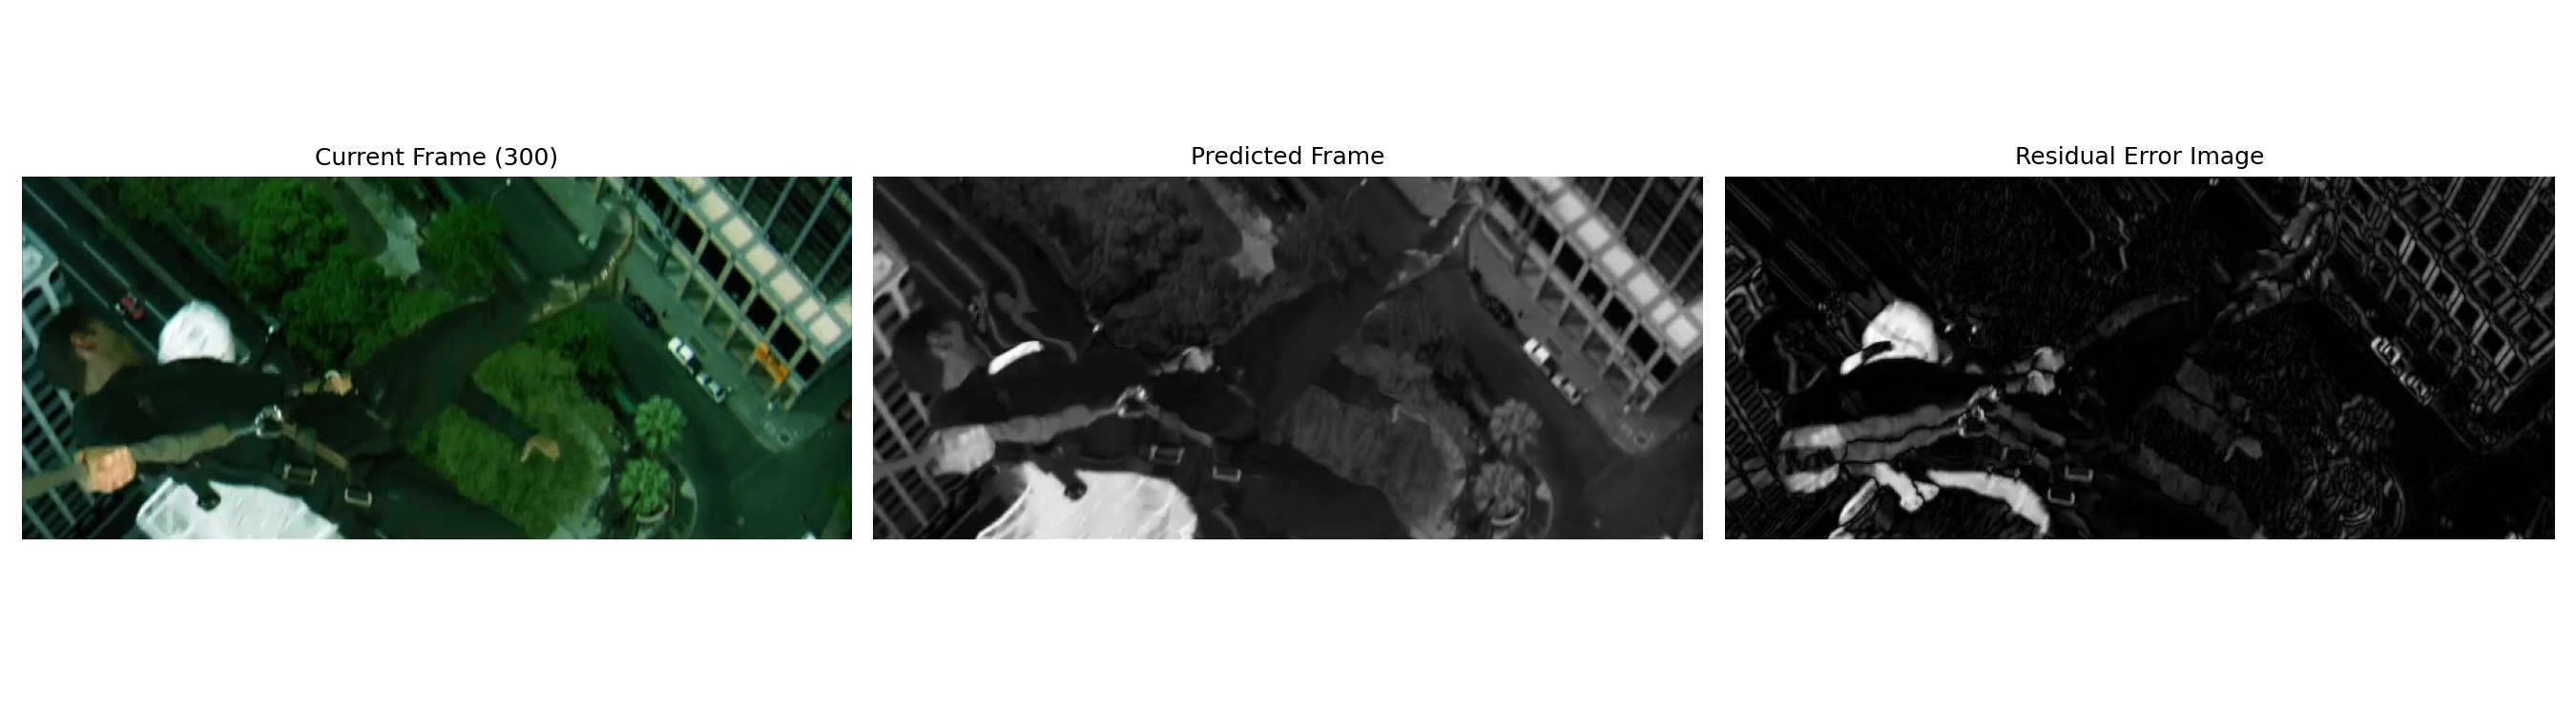
\includegraphics[width=\textwidth]{Images/q3_matrix_residual.png}
        \caption{Exemple d’image résiduelle pour la vidéo Matrix.}
    \end{figure}
    
    Cette séquence produit de très bons résultats.  
    Les changements de plans génèrent des résidus très marqués tandis que les mouvements internes aux scènes restent relativement cohérents.
    
    \subsection*{Mesures statistiques}
    
    Afin de détecter automatiquement les changements de plans, plusieurs mesures statistiques ont été calculées :
    
    \begin{itemize}
        \item la moyenne des erreurs résiduelles ;
        \item l’entropie de l’image résiduelle ;
        \item la différence entre histogrammes successifs.
    \end{itemize}
    
    \subsubsection*{Entropie des résidus}
    
    L’entropie des images résiduelles est calculée à partir de l’histogramme des intensités :
    
    \[
    H(R_t)= - \sum_i p_i \log_2(p_i)
    \]
    
    où $p_i$ représente la probabilité d’apparition du niveau de gris $i$ dans l’image résiduelle.
    
    \vspace{0.3cm}
    
    Une forte entropie indique généralement :
    \begin{itemize}
        \item un changement important dans la scène ;
        \item une mauvaise prédiction par flot optique ;
        \item ou un changement de plan potentiel.
    \end{itemize}
    
    \subsection*{Détection des changements de plans}
    
    Le détecteur final combine plusieurs critères :
    
    \begin{itemize}
        \item une forte entropie résiduelle ;
        \item une différence importante entre histogrammes successifs ;
        \item une contrainte temporelle évitant plusieurs détections consécutives.
    \end{itemize}
    
    Les figures suivantes présentent l’évolution temporelle des différentes mesures statistiques.
    
    \begin{figure}[H]
        \centering
        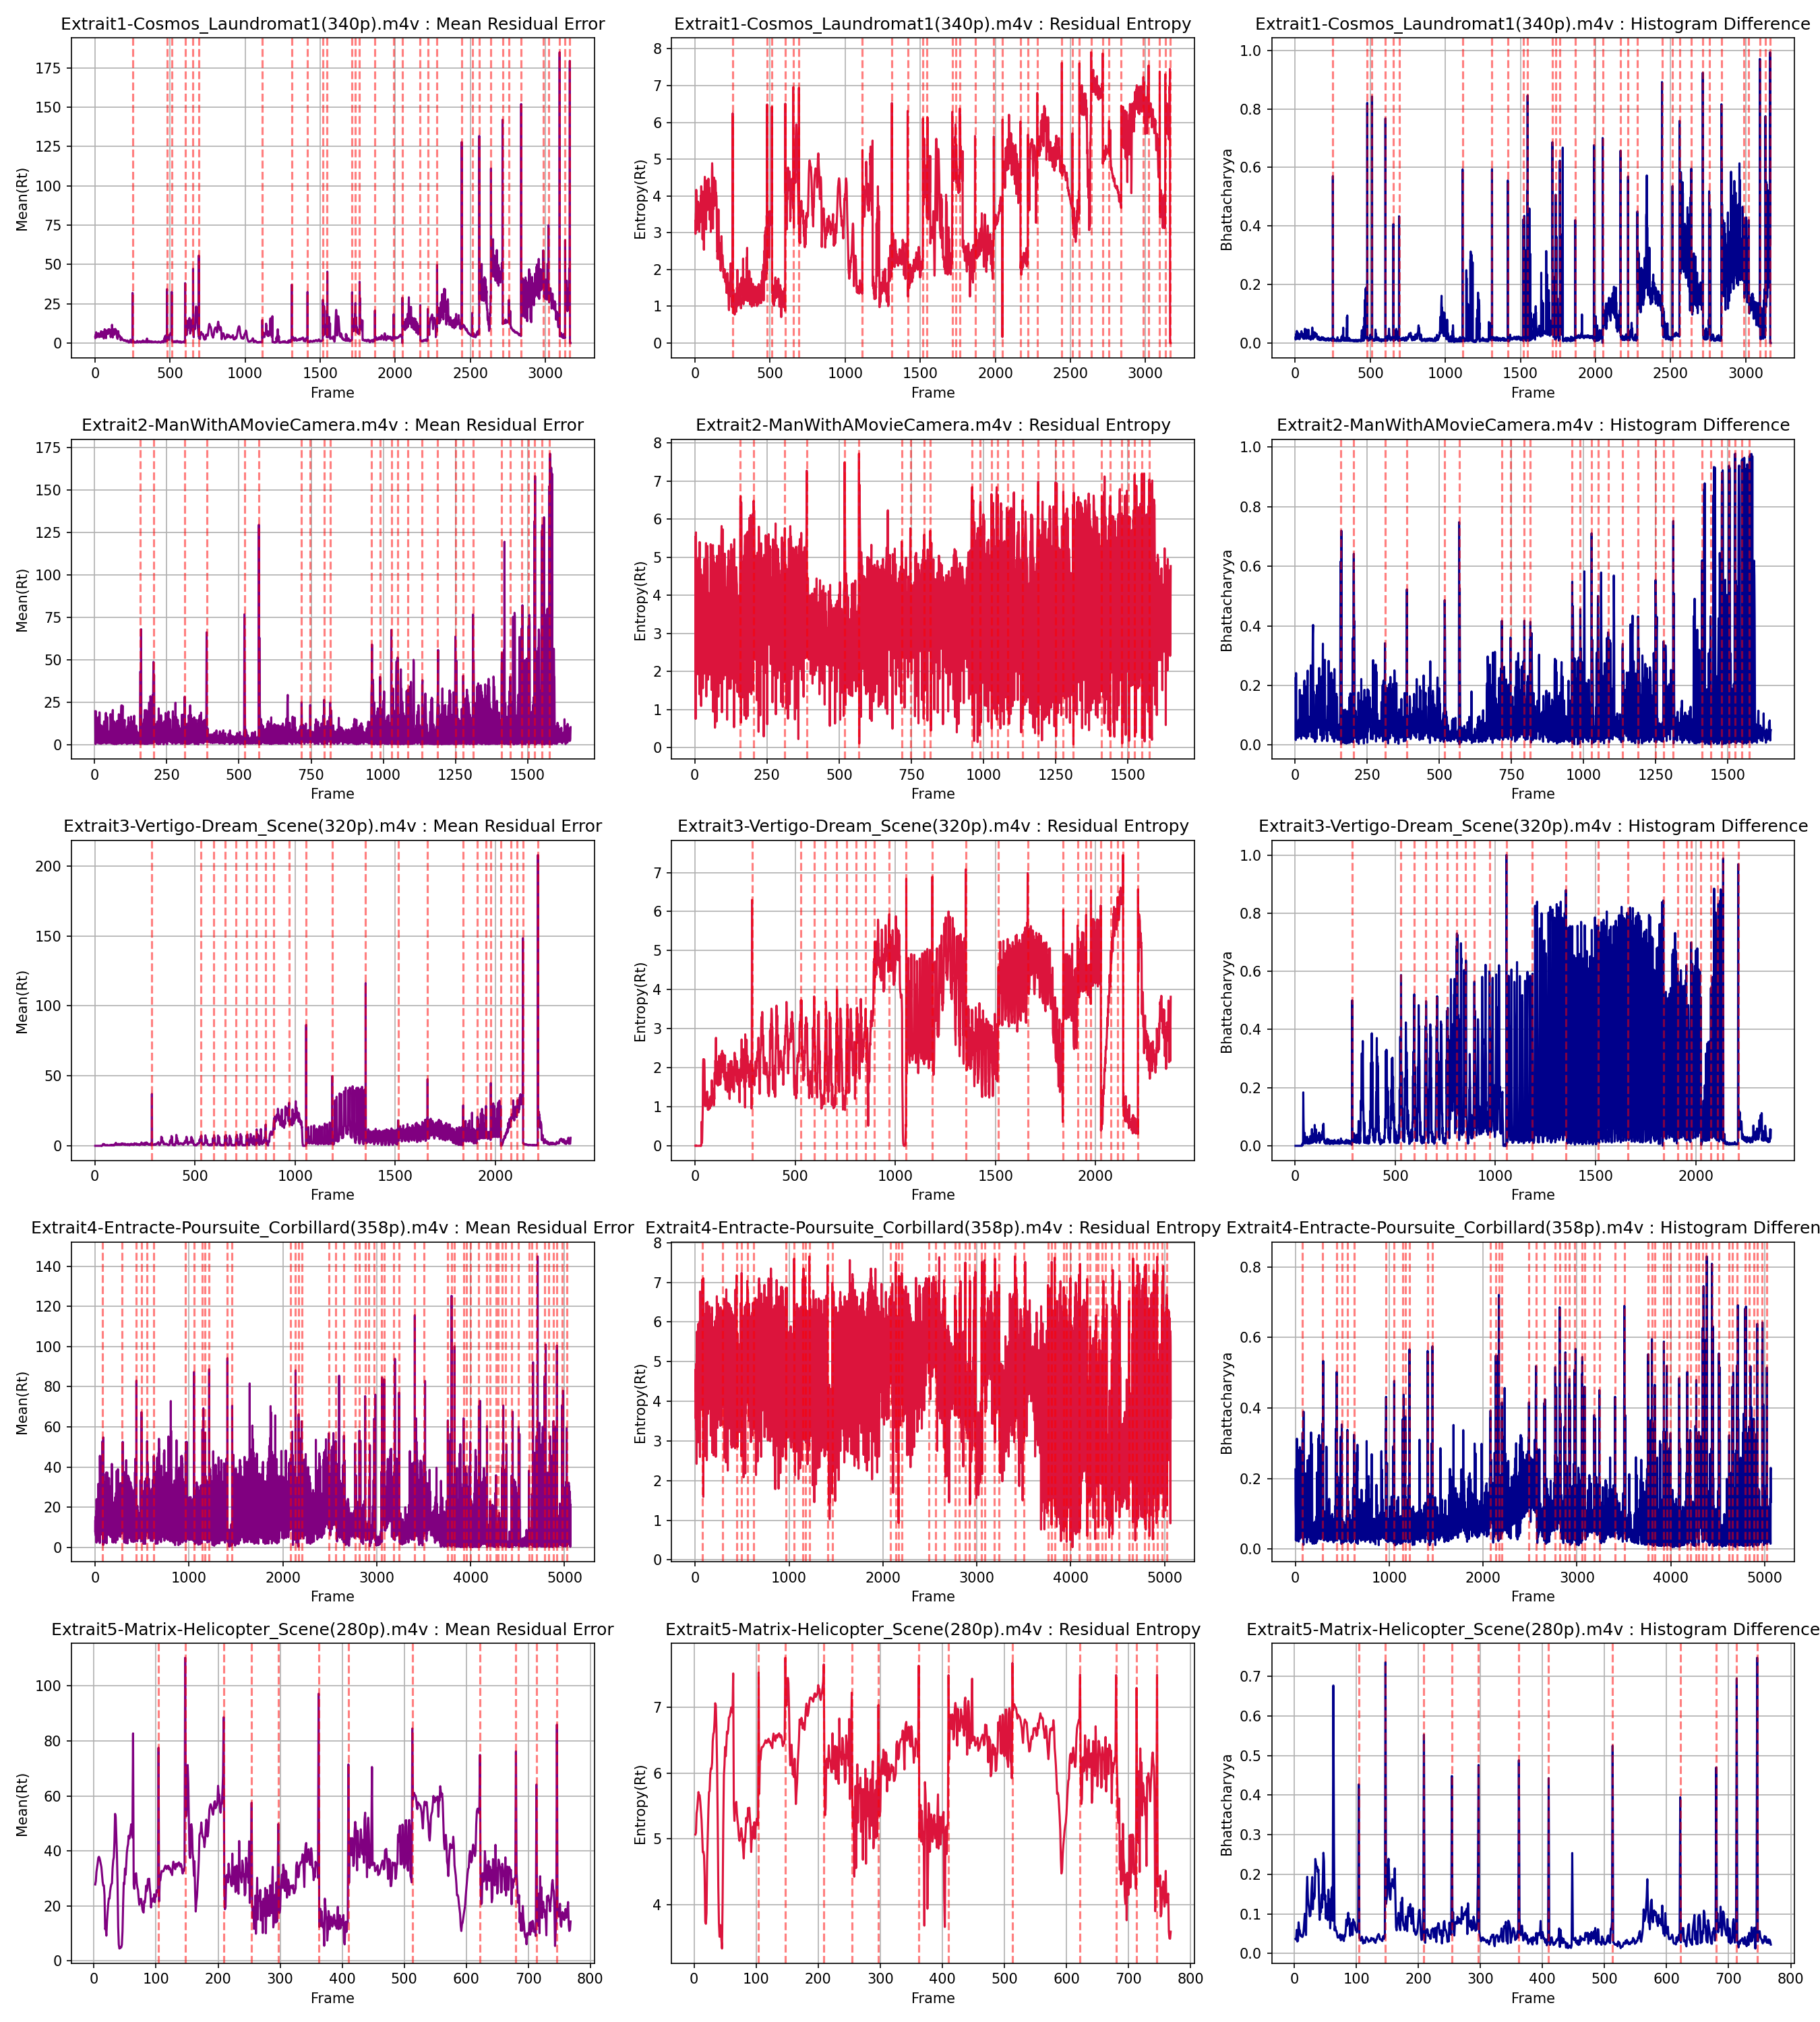
\includegraphics[width=\textwidth]{Images/q3_statistics.png}
        \caption{Évolution temporelle des mesures statistiques utilisées pour la détection des changements de plans.}
    \end{figure}
    
    Les lignes verticales correspondent aux changements de plans détectés automatiquement.
    
    \subsection*{Analyse des résultats}
    
    Les résultats obtenus sont globalement satisfaisants :
    
    \begin{itemize}
        \item les vidéos 1 et 5 présentent une très bonne détection des changements de plans ;
        
        \item les vidéos monochromes restent plus difficiles à traiter en raison de l’absence d’information chromatique ;
        
        \item la vidéo 3 génère plusieurs faux positifs à cause des changements rapides de couleurs et des effets lumineux ;
        

    \end{itemize}
    
    \subsection*{Limites de la méthode}
    
    Plusieurs difficultés apparaissent lors de l’utilisation du flot optique pour la détection des changements de plans :
    
    \begin{itemize}
        \item mouvements rapides de caméra ;
        
        \item effets de clignotement lumineux ;
        
        \item flou de mouvement ;
        
        \item bruit présent dans les anciennes vidéos monochromes ;
        
    \end{itemize}
    
    De plus, certaines variations importantes d’éclairage peuvent produire des résidus élevés sans correspondre à un véritable changement de plan.
    
    \subsection*{Conclusion}
    
    Cette étude montre que l’analyse des images résiduelles constitue une méthode efficace pour détecter les changements de plans dans des séquences vidéo.
    
    La combinaison :
    \begin{itemize}
        \item du flot optique ;
        \item de l’entropie des résidus ;
        \item et des différences d’histogrammes
    \end{itemize}
    
    permet d’obtenir des résultats robustes sur plusieurs types de vidéos.
    
    \vspace{0.3cm}
    
    Malgré certaines limitations, cette approche fournit une représentation pertinente des discontinuités temporelles présentes dans les séquences vidéo.
    
\end{document}
